\RequirePackage[hyphens]{url}
\documentclass[11pt,titlepage,dvipsnames,table,xcdraw]{article}
\usepackage{strath-dissertation}
\usepackage{setspace}
\usepackage{geometry}

\geometry{a4paper,portrait,margin=2.5cm}


\usepackage{babel}
\usepackage{lipsum} % For demonstration only.

%--------------------------------
% Degree settings
%--------------------------------
\newcommand{\degreename}{Bachelor of Science}
\newcommand{\coursename}{CS408: Individual Project}
\newcommand{\deptname}{Computer and Information Sciences}

\usepackage{amsmath} % fix stupid warning
\usepackage{amssymb}
\usepackage{sansmathfonts}
\usepackage{slantsc}

\renewcommand{\familydefault}{\sfdefault}
\DeclareFontSeriesDefault[sf]{bf}{bx}

% Define code block styling
%
\usepackage{color}
\definecolor{lightgray}{rgb}{.9,.9,.9}
\definecolor{darkgray}{rgb}{.4,.4,.4}
\definecolor{purple}{rgb}{0.65, 0.12, 0.82}

% Traceability table styling (Product section).
\usepackage{booktabs}
% Allows the [H] specifier to pin a figure exactly in reading order.
\usepackage{float}
% Side-by-side sub-figures with their own captions.
\usepackage{subcaption}
% Floats on float-only pages sit at the top instead of being vertically
% centred (the article class default stretches equal glue above and below).
\makeatletter
\setlength{\@fptop}{0pt}
\makeatother
\newcommand{\statusmet}{\textcolor{OliveGreen}{Met}}
\newcommand{\statuspartial}{\textcolor{BurntOrange}{Partial}}
\newcommand{\statusdeferred}{\textcolor{gray}{Deferred}}
\lstdefinelanguage{Typescript-min}{
  keywords={break, case, catch, continue, debugger, default, delete, do, else, false, finally, for, function, if, in, instanceof, new, null, return, switch, this, throw, true, try, typeof, var, void, while, with, type, let, const},
  morecomment=[l]{//},
  morecomment=[s]{/*}{*/},
  morestring=[b]',
  morestring=[b]",
  ndkeywords={class, export, boolean, throw, implements, import, this },
  keywordstyle=\color{blue}\bfseries,
  ndkeywordstyle=\color{darkgray}\bfseries,
  identifierstyle=\color{black},
  commentstyle=\color{purple}\ttfamily,
  stringstyle=\color{red}\ttfamily,
  sensitive=true
}
% Style for short shell commands: grey box, prompt marker, no line numbers.
\lstdefinestyle{shellcmd}{
  language=bash,
  backgroundcolor=\color{lightgray},
  basicstyle=\ttfamily\small,
  numbers=none,
  frame=single,
  framerule=0pt,
  xleftmargin=6pt,
  xrightmargin=6pt,
  aboveskip=8pt,
  belowskip=8pt,
  breaklines=true,
  showstringspaces=false,
  keywordstyle=\color{black},
  stringstyle=\color{black},
  identifierstyle=\color{black},
  prebreak=\raisebox{0ex}[0ex][0ex]{\ensuremath{\hookleftarrow}}
}
\begin{document}

%--------------------------------
% Title page.
%--------------------------------
\begin{titlepage}
\vspace{5mm}
\titletext{Improving Automated Assessment}
\vspace{10mm}
\authortext{Michal Skraburski}
\vspace{15mm}
\degreetext{\degreename}{\coursename}
\vspace{40mm}
\centredcrest
\vspace{5mm}
\depttext{\deptname}
\vspace{5mm}
\datetext{August, 2026}
\end{titlepage}

%--------------------------------
% Front matter numbering.
%--------------------------------
\pagenumbering{roman}
\setcounter{page}{2}

%--------------------------------
% Setting counter depth.
%--------------------------------
\setcounter{secnumdepth}{3}
\setcounter{tocdepth}{3}

%--------------------------------
% The front matter.
%--------------------------------
\setstretch{1.2} % 1.5 line spacing. 

%Abstract

%    Introduction
%    Background Literature
%    Specification & Design
%    Implementation
%    Evaluation
%    Results
%    Discussion & Reflection
%    Future Work
%    Conclusion

%References
%Appendices-


\begin{abstract}

CodeRunner, the Moodle question type used to set and automatically grade programming exercises at the University of Strathclyde and elsewhere, is a mature and capable tool whose remaining weaknesses are problems of experience rather than of capability. Authoring a question means working through a dense editing form with fixed test-case batches, help text that vanishes on a click and misaligned controls, while its documentation is a single feature-organised page; students answer through a fixed layout with hidden feedback and little room to work. This project treated those frictions as an engineering problem and set out to remove them without disturbing what already worked.

The work proceeded from evidence to delivery. CodeRunner and its two audiences were analysed through heuristic review, interviews and a survey of students and teachers; the faults found were turned into prioritised requirements; and the improvements were built inside a fully reproducible Docker development environment that recreates the whole system with a single command. The delivered changes span both sides of the tool: flexible test-case management and a corrected Precheck display for authors, a switchable and resizable layout and reclaimable space for students, measurable accessibility gains, and task-focused documentation, with in-plugin search, served from within the plugin and reachable from the editing form.

The changes were verified by twenty-seven unit tests and the plugin's own browser-driven regression suite, all of which pass, and their value was confirmed by the survey: every delivered feature won majority approval from both students and teachers, no feature was rejected, and the accessibility audit rose from 93\% to 97\%. The significance of the result is methodological as much as practical: it demonstrates that a widely deployed educational tool can be improved meaningfully by disciplined user-experience engineering on the existing system, rather than by building a replacement.

\end{abstract}





%\input{sections/declaration}
\clearpage
\section*{Acknowledgements}

I would like to thank the participants who evaluated my project designs, my supervisor Andrew Fagan, the friends and family who supported me throughout.







  % Uncomment to include this page.

%--------------------------------
% Tables of contents.
%--------------------------------
\setstretch{1.0} % 1.0 line spacing.  
\clearpage
\tableofcontents
%\listoffigures   % Uncomment for a list of figures.
%\listoftables    % Uncomment for a list of tables.
\clearpage

%--------------------------------
% The body of the document.
%--------------------------------
\pagenumbering{arabic} % Page numbering for rest of document.
\setstretch{1.5} % 1.5 line spacing. 
\section{Introduction}

Universities teach programming to cohorts far larger than any team of markers can assess by hand, and automated assessment has become the standard answer: students submit real code, the code is run against tests, and a grade is produced in seconds~\cite{reviewrecentsystems2010}. At the University of Strathclyde this happens inside Moodle, the online learning platform behind MyPlace, through a plugin called CodeRunner~\cite{CodeRunner2016}. CodeRunner adds a new kind of quiz question: one answered by writing a program, which is compiled, executed and graded automatically. It is mature, widely deployed and, in terms of raw capability, largely complete.

Capability, however, is not the same as usability. The lecturers who author CodeRunner questions face a dense editing form offering a full suite of tools with little guidance on how to use them: test cases can be added only in fixed batches and never deleted, help text vanishes the moment it loses focus, controls sit misaligned, and the official manual is a single enormous page organised around the system's features rather than the author's task. The students answering questions have their own frictions: a fixed layout that forces scrolling between the question and the answer, screen space consumed by margins and panels, hidden tests that give zero details why they fail and no modern LSP support -- using the CodeRunner page for writing and testing code execution is doom for the students' grade. None of these faults stops anyone using the tool. Each one, multiplied across every question authored and every answer written by thousands of users, quietly taxes teaching and learning alike. Well-established design principles hold that this kind of friction is a software problem rather than a user problem~\cite{designofeveryday}, and tools embedded in education must keep evolving to meet its growing demands~\cite{pieterse2013automated}.

This project set out to remove that friction. The problem was approached as a user experience engineering task on a live, mature codebase: understand the system and its two audiences, identify the faults with evidence rather than intuition, turn the evidence into requirements, and deliver the improvements without breaking anything that already worked. Concretely, the project analysed CodeRunner through heuristic review, a survey of students and teachers, and interviews; built a fully reproducible Docker-based development environment in which the entire system can be recreated with one command; and delivered a set of improvements spanning both pages: proper test case management for authors, a corrected Precheck display, a switchable and resizable question layout, reclaimable screen space, measurable accessibility gains, and task-focused documentation served from inside the plugin itself. The changes were verified with unit and browser-driven acceptance tests, and the delivered features were subsequently confirmed to be worth building by the survey, whose results are reported in Section~\ref{results}.

The project's objectives were:

\begin{description}
\item [Objective 1:] Construct an isolated, repeatable development environment in which Moodle, CodeRunner and its dependencies can be built, run and regression-tested with minimal effort.
\item [Objective 2:] Improve the ergonomics of the author page: flexible test case management, correct rendering, visual consistency and measurable accessibility.
\item [Objective 3:] Improve the student answering experience: control over the question layout, reclaimable screen space and the ability to save work on demand.
\item [Objective 4:] Provide effective, task-focused documentation reachable from within the tool.
\item [Objective 5:] Evaluate the delivered changes with real students and teachers, and derive further requirements from their feedback.
\end{description}

The remainder of this dissertation follows the project's own course. Section~\ref{backg} reviews the literature that informed it. Section~\ref{process} describes the methodology, the analysis of CodeRunner and its users, the requirements that emerged, and the designs that answered them. Section~\ref{product} details the implementation of each change and the verification and validation performed. Section~\ref{results} presents the survey results and their evaluation. The report closes with a discussion of the findings, an honest reflection on the process, and the conclusions drawn from the work.
 % Add one file per section.
\clearpage
\section{Background Literature}\label{backg}

This section reviews the literature that informed the project, in four strands: the state of automated programming assessment, the field's persistent weakness in feedback, the design principles used to evaluate and improve the interfaces, and the standards and practices that shaped the engineering. Each strand ends where the project begins, and the review closes by positioning the project against them.

\subsection{Automated Assessment of Programming}

Assessing programming by hand does not scale, and it barely works even when it is affordable: Lobb and Harlow open the CodeRunner paper by observing that hand-written code on paper is nearly impossible to grade meaningfully, because static reading cannot reveal whether a student could make their program actually run~\cite{CodeRunner2016}. The field's answer, developed over decades, is to execute submissions against instructor-defined test cases and grade the outcome. Ihantola et al.'s systematic review of assessment systems shows both the maturity and the fragmentation of this space: dozens of tools exist, most built around the same test-based core, differing in how teachers define tests, how resubmission is handled, and how securely untrusted code is run~\cite{reviewrecentsystems2010}. Two of that review's conclusions matter here. First, test-based assessment is the settled approach; CodeRunner is an orthodox member of the family. Second, the authors explicitly criticise the field's habit of building yet another new system, and encourage opening up and extending the systems that already exist. That recommendation is a direct argument for the shape of this project: improving a widely deployed tool rather than producing a new one.

Pieterse's analysis of automated assessment adds the operational perspective: the success of such systems depends on factors beyond grading correctness, including how students experience failure and how much confidence teachers have in the tool, and the requirements placed on these systems grow as education leans harder on them~\cite{pieterse2013automated}. A tool can therefore be complete in capability yet still fall short of what its users need, which is precisely the position this project found CodeRunner in.

\subsection{The Feedback Problem}

The most consistent criticism in the assessment literature concerns feedback. Keuning, Jeuring and Heeren's systematic review of automated feedback generation finds that most tools report whether a submission is correct but offer little help with why it failed or how to move forward~\cite{keuningfeedback}. This is the academic form of the complaint that surfaced independently in this project's survey: hidden test cases fail without telling the student what went wrong, leaving them to guess at the cost of further penalty. The literature thus both anticipates the pain point and elevates it from an anecdote to a known, field-wide weakness, which is why hints for hidden test cases (FR5) is treated as the highest-value item of future work rather than a passing suggestion.

A newer strand asks whether large language models can close the feedback gap. Phung et al.\ benchmark ChatGPT and GPT-4 against human tutors across programming education tasks, including grading, and find that even the strongest models approach but do not match human tutors~\cite{llmgrading}. For grading specifically, where consistency is a fairness requirement, approaching is not enough; this evidence underpins the decision, discussed in Section~\ref{process}, to consider and exclude LLM-based grading from the project's scope.

\subsection{Usability and Design Principles}

The project's central claim, that CodeRunner's remaining problems are experience problems, rests on established design literature. Norman's \emph{The Design of Everyday Things} argues that what is habitually called user error is usually design error: systems that punish slips, hide their state, or demand documentation to operate are failing their users, not the reverse~\cite{designofeveryday}. Norman also supplies the vocabulary of affordances, controls whose appearance invites their use, which this project applies directly in the design of its student-facing controls. Krug's \emph{Don't Make Me Think} distils the same stance for the web: an interface should be self-evident, and every moment a user spends puzzling over a control is a cost paid for a design decision~\cite{dontmakemethink}. These two works served as the lenses for the heuristic review of CodeRunner's pages reported in Section~\ref{process}.

Written guidance is part of the interface as well. Google's developer documentation style guide asks writers to organise content around the reader's task, keep pages short and scannable, and explain no more than the task requires~\cite{googledevstyle}. It was used as the yardstick for CodeRunner's documentation, and the requirement it produced (NFR3) is essentially the guide's advice turned into an acceptance criterion.

\subsection{Standards and Engineering Practice}

Accessibility work in this project is anchored to two W3C standards: the Web Content Accessibility Guidelines define what an accessible page must achieve~\cite{w3c_wcag22_2023}, and WAI-ARIA defines the vocabulary of attributes used to achieve it in rich interfaces, including the labelling and live-region techniques applied here~\cite{w3c_wai_aria12_2023}. The Lighthouse audit used to measure progress derives its accessibility checks from these guidelines, which makes the requirement NFR2 measurable rather than aspirational.

The engineering practices around the product likewise follow the literature. Docker's containerisation, packaging applications with their dependencies into isolated and reproducible units~\cite{dockerjournal}, is what makes the development environment requirements (DE1 and DE2) satisfiable with one command. Behaviour-driven development, as introduced by North, frames acceptance tests as executable descriptions of behaviour~\cite{northbdd}; CodeRunner's upstream Behat suite is exactly such a description, and running it unmodified is this project's regression evidence. The survey instrument was designed with reference to Kitchenham and Pfleeger's principles of survey research in software engineering~\cite{designingsurvey}, and the validation of requirements against implementations follows the traceability practice analysed by Gotel and Finkelstein~\cite{goteltraceability}.

\subsection{Positioning of this Project}

Read together, the strands position the project precisely. The assessment literature says the grading problem is solved and advises improving existing systems over building new ones; the feedback literature identifies experience, not capability, as the open weakness; the design literature supplies principles and methods for fixing experience problems and insists such problems belong to the software; and the standards make the improvements measurable. This project sits at that intersection: an evidence-driven user experience improvement of a mature, widely used automated assessment tool, evaluated with its real users.
 % Add one file per section.
\clearpage

\section{Specification \& Design}\label{process}
This section describes how the project took shape: how CodeRunner and its place inside Moodle (the platform behind Strathclyde's MyPlace) came to be understood, how the state of the system was assessed, and how that assessment turned into a concrete set of requirements and designs. The work began by picking the system apart to learn how it operates: its components, its dependencies, and how they fit together. Its features were then inspected with a critical eye, hunting for flaws, bugs and missing functionality, with the opinions of real users gathered as a check on the analysis.

Doing any of this needed somewhere safe to experiment, so the first step was building a fresh, self-contained copy of the entire system: a Dockerized Moodle with CodeRunner and its dependencies integrated into it, plus scripts that automate compiling and testing. The four codebases involved -- CodeRunner, its companion behaviour plugin, the Dockerized Moodle and this dissertation -- live together in one shared repository (a monorepo), which kept the moving parts easy to manage as one project.

CodeRunner is a mature and largely feature-complete system, so the project's focus fell naturally on user experience: analysing, modifying and polishing the pages that lecturers and students actually touch. The features chosen for development came from the analysis and were confirmed to be worth building through a survey. The remainder of this section covers the methodology followed, the analysis itself, the requirements that emerged from it, and the designs that answered them.


\subsection{Methodology}
The project followed a technique similar to Agile (single 2-week sprint).
Development ran as a closed feedback loop: upon a feature reaching a good state, opinions were requested from peers and the project supervisor, alongside consulting the literature reviewed in Section~\ref{backg}.
This technique was chosen specifically because it fits an iterative style of design better than the other options. It also serves UI design well, as it benefits from a constant feedback loop.

\subsection{Analysis}

\subsubsection{Understanding the System}
It is first necessary to understand CodeRunner, its operation, and its integration with the wider Moodle platform. This was done by looking at the project, cloning the repo to the development environment and setting it up. Moodle itself is the core: an online education platform used by universities to host courses, quizzes and teaching material, which allows modification by plugins, add-on packages that can alter scripts, override behaviour and styles, and add functionality. CodeRunner is a plugin which augments itself onto the list of available question types~\cite{CodeRunner2016}. For example, a multiple choice question and a text entry question are both question types; CodeRunner expands this list of question types by one: a question answered by writing a real computer program, graded automatically by running it against test cases, example inputs paired with the outputs the lecturer expects, the approach taken by most automated assessment systems~\cite{reviewrecentsystems2010}. CodeRunner extends the question framework through a required dependency, \texttt{qbehaviour\_adaptive\_adapted\_for\_coderunner} (Figure~\ref{fig:dependency_graph}). This required plugin is the railway for sending input, defining and managing the types of submission and their results (such as a Precheck, a trial run that lets a student check their code without spending marks); CodeRunner itself is the station for this railway, managing the interaction between Jobe (a separate, sealed-off server whose only job is to compile and run the code students submit, keeping untrusted code out of Moodle itself; deployed here as the ready-made Jobeinabox package) and the now-overridden types of results. CodeRunner extends the author page (where a lecturer builds a question) and the student question page (where a student answers it) through Moodle's standard extension points to add its functionality, as per the Moodle plugin dogma.

\begin{figure}[h]
    \centering
    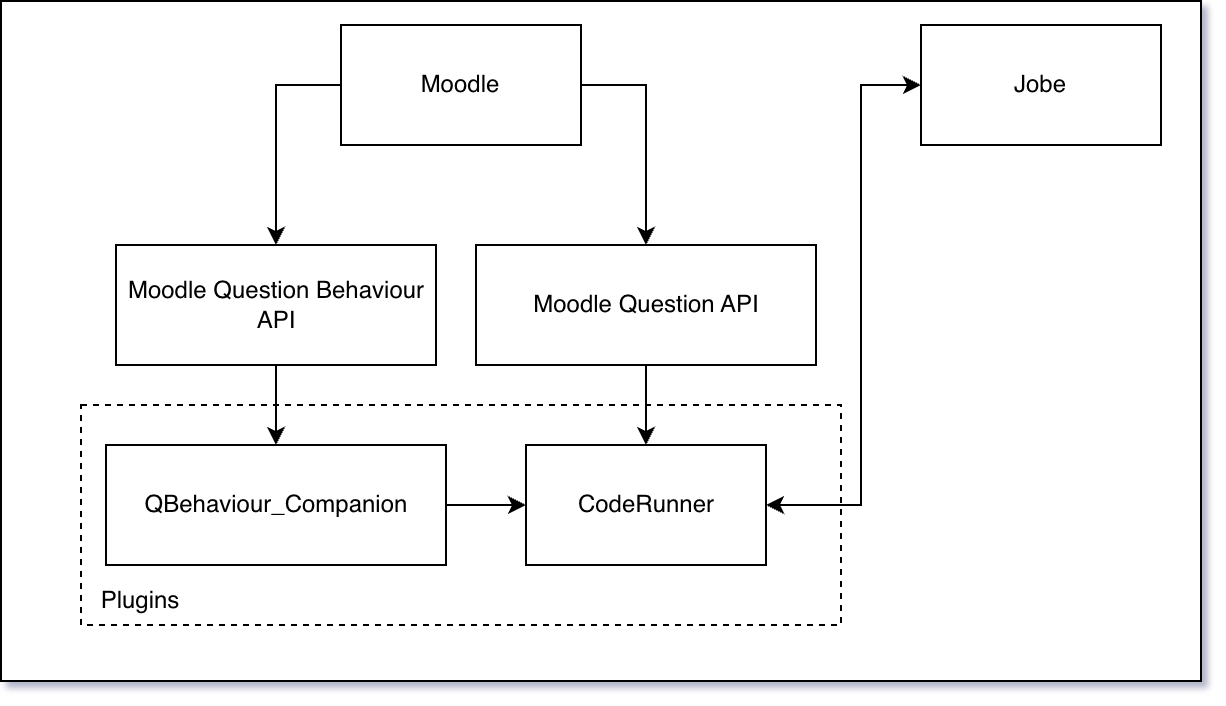
\includegraphics[width=0.8\textwidth]{figs/dependency_graph.png}
    \caption{Moodle \& Plugin dependency graph}
    \label{fig:dependency_graph}
\end{figure}

\subsubsection{Environment Setup}
After figuring out the project, the work turned to Docker: software that packages a program together with everything it needs into isolated `containers', so that the same setup runs identically on any machine~\cite{dockerjournal}. Due to a lack of knowledge, Docker had to be learned for the first time; however this allowed a much faster setup and an automatically repeatable environment.
This allowed Moodle to run, but not CodeRunner yet, because the in-development copies of the plugins had to be connected into the running Moodle (using Docker's bind mounts, which share a folder on the host machine with a container). This did not work as planned because the strict permissions of the macOS laptop used for development stopped the shared folders from working properly. Once this was realized, development switched to a desktop machine running Linux, which fixed the issue.
The project still did not work because Moodle's strict security policy blocks the web requests its components use to talk to one another (cURL requests), even local ones between Docker containers. Allowing these was required because one of the CodeRunner dependencies is Jobeinabox, the code-running server described above. This was not obvious at the time, and many hours were spent trying to figure out what was wrong with the Docker setup.

\subsubsection{Problem Identification}
The project was analysed by researching what issues CodeRunner has:
searching the public repository for posted issues, fielding a survey, interviewing lecturers, requesting fellow students' opinions, and including first-hand observations from using the system.
It quickly became clear that what had been presumed to be a lecturer problem was actually a software problem. User design books like Don Norman's \emph{The Design of Everyday Things}~\cite{designofeveryday} show that user error often isn't the user's fault. In the case of CodeRunner this was and still is absolutely correct. CodeRunner is one of the many software tools that will forever need to evolve due to the growing requirements of education~\cite{pieterse2013automated}.

\subsubsection{Review of the Author Page}
The existing design for both student facing and author facing pages was reviewed against the design literature introduced in Section~\ref{backg}: Don Norman~\cite{designofeveryday} and \emph{Don't Make Me Think} by Steve Krug~\cite{dontmakemethink} for the interfaces themselves, and Google's developer documentation style guide~\cite{googledevstyle} as the yardstick for the written documentation. 

The author page explains the frustration felt towards lecturers: the user experience provides a full suite of tools with no instructions on how to use them properly. A long single page document can be found on the CodeRunner documentation \cite{coderunnergitiodocs}, and it is extremely well-written and complete; however, it falls short of Google's guidance, which asks writers to organise content around the reader's task, to keep pages short and scannable, and to avoid explaining more than the task at hand requires. The CodeRunner manual does the opposite on each count: it is organised around the system's features, lives on one enormous page, and explains far more than the basic user needs. It is as though IKEA sent you a wardrobe with instructions on how to build every single type of wardrobe in their catalog and it is up to you to figure out which instructions you need to follow. This assessment directly shaped the documentation requirement (NFR3) and the task-focused documentation page later built to satisfy it.

\begin{figure}[h]
    \centering
    \setlength{\fboxsep}{0pt}%
    \fbox{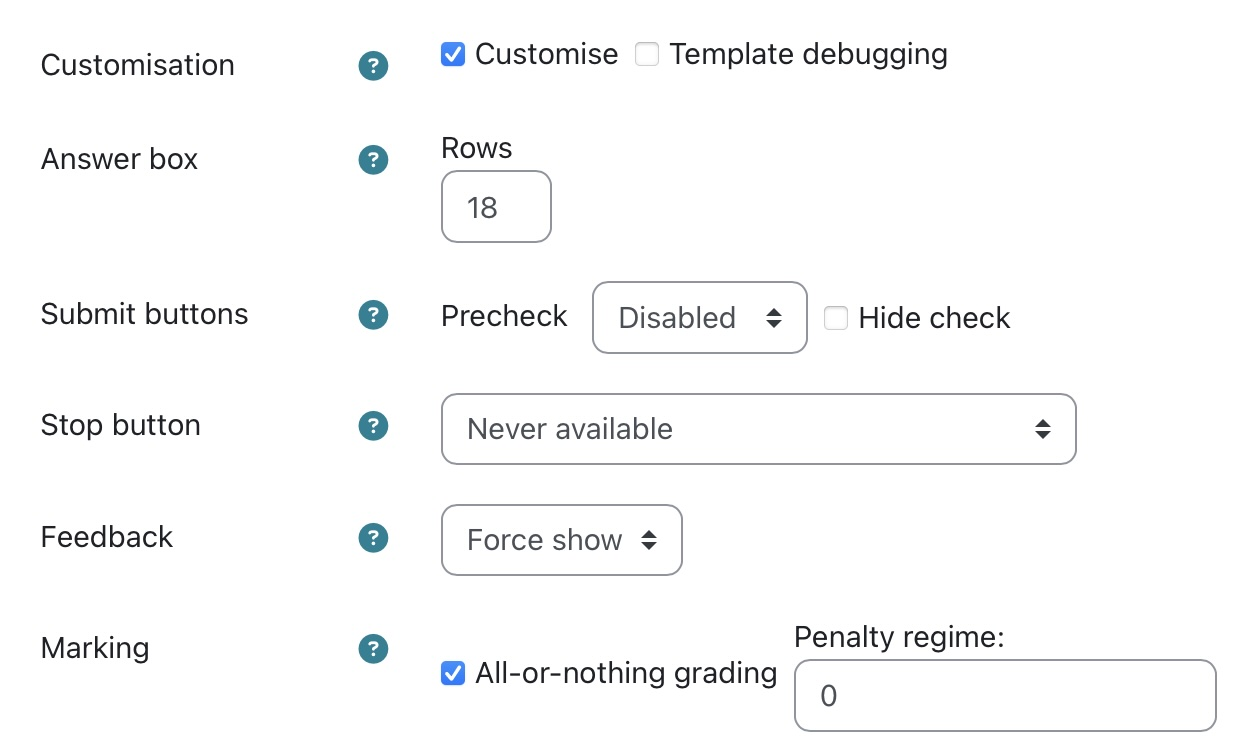
\includegraphics[width=\dimexpr\linewidth-2\fboxrule\relax]{figs/authorpage_1.jpg}}
    \caption{The CodeRunner author page's question-option controls, showing the per-label help buttons and the inconsistent label alignment discussed in this section.}
    \label{fig:authorpage_1}
\end{figure}

The author page (Figure~\ref{fig:authorpage_1}) is rough around the edges, and the burrs show on test cases: you can only add 3 test cases per request, no more no less. You also can't delete the excess test cases. The user interface as a whole is also very dense, jumbled and indecisive; some labels appear above their selectors, some appear to the left of them. Checkboxes scattered across the page, misaligned with their labels also. The corners of the test case boxes are also completely square, unlike every other box on the page, which are all rounded. Every help button beside every major label does nothing aside from opening one large column of text that explains what the feature does, but it disappears the moment you click elsewhere, and the text is difficult to read properly because it can overflow due to length (Figure~\ref{fig:authorpage_helpoverflow}). 

\begin{figure}[H]
    \centering
    \setlength{\fboxsep}{0pt}%
    \fbox{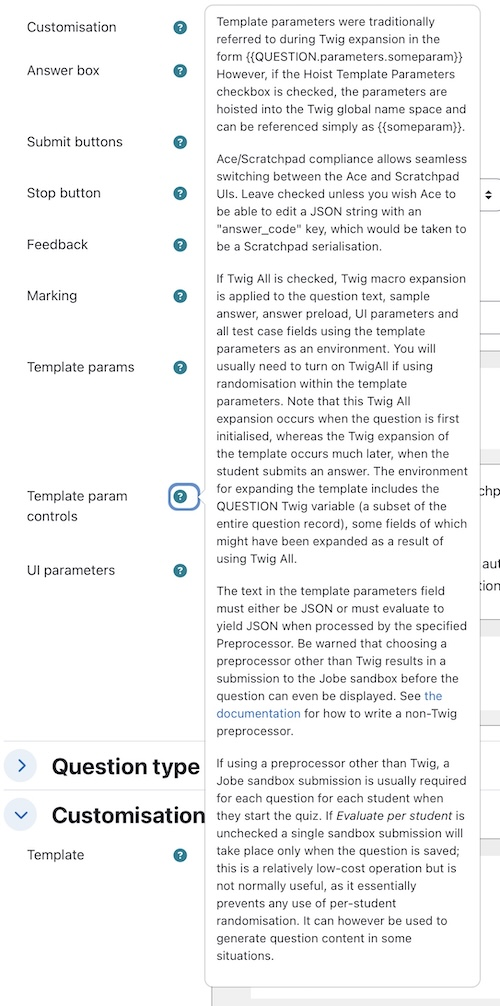
\includegraphics[height=0.55\textheight]{figs/authorpage_helpoverflow.jpg}}
    \caption{Author page showing the almost overflowing help hint discussed.}
    \label{fig:authorpage_helpoverflow}
\end{figure}

When the Precheck option is enabled, it appears in the label column of the test case instead of the input column to its right, and the padding of the row above separates it visually from the test case box it belongs to, appearing disjointed. A Lighthouse audit (an automated page-quality check built into the Chrome browser) scores this page at only 93\% for accessibility, a measure of how usable a page is for people relying on assistive tools such as screen readers, instead of the preferable 100\%: several of the input controls in CodeRunner lack ARIA labels (invisible text that a screen reader speaks aloud), as does the Ace Editor, the code-editing box embedded in the page. Despite the author page being very technically heavy, there are very few self-explanatory options; the help buttons make some of them self-evident, but they often fail to explain how the question lifecycle really works \cite{dontmakemethink}.

\subsubsection{Review of the Student Page}
The student-facing question answer page is polished and complete. This page is quite good when the author writes the questions correctly; for example, a bad question would be where the question description is too massive to view both the description and the answer box at once. Another example is when the author chooses to use hidden test cases (tests whose details are concealed from the student, so that answers cannot simply be written to pass them): this is good for the author but it does not help the student at all. Often an author will have many hidden test cases and it is unknown which one the student failed, especially under complex questions. Inspection of the code showed that a written answer in the page is only saved automatically every 60 seconds, in the background; while this is acceptable, the user might benefit from an affordance (in Don Norman's sense~\cite{designofeveryday}, a control that visibly invites its use) which allows them to save manually.

\subsubsection{Survey Analysis}

Furthermore, pursuing a survey, designed with reference to established principles of survey research~\cite{designingsurvey}, yielded further requirements and analysis. A list of comments and suggestions follows:
\begin{itemize} 
  \item `I don't like that hidden test cases don't tell the user where they went wrong', paraphrased, in reference to student-facing page, the system currently does not tell the student why they failed a hidden test case within a question.
  \item `A hint option that deducts marks if used' in reference to the student-facing page, the system should allow the user to get hints in exchange for a reduced mark.
    This option is very similar to giving hints on hidden test cases failed instead of silently erroring out.
  \item `An LLM to check whether the answer is close enough may be beneficial as CodeRunner often expects unrealistically exact inputs/outputs.' in reference to the grading methods available.
  \item `An attached command terminal for outputs would be useful for interactive prototyping.' in reference to the student-facing page, it shall allow the user to run custom commands and tests.
  \item `It would be nice if it had LSP support.' in reference to the editor, the idea is to extend the editor's ability to flag errors and runtime errors prior to the answer being checked.
  \item `Provide commands such as the gcc line which could be copied into a clipboard' paraphrased, in reference to the student-facing page, the question should provide a codebox which allows the user to click a copy button instead of selecting and copying it manually.

\end{itemize}

In the order listed above, the following discusses the viability and benefit-to-cost ratio of each suggestion.

Providing a hint button is an idea very similar to allowing the user to get more information out of hidden test cases; the latter is arguably the bigger problem because in most cases the questions the lecturers write are well detailed and more than enough. The issue with hidden test cases is that often the student can be left guessing what is wrong instead of getting a detailed answer as to why they are failing, which costs them even more penalty if they guess wrong. In the real world, a developer can usually find a reason as to why something in their code isn't working correctly.

An LLM (large language model, the technology behind tools such as ChatGPT) addition to the question grading options is an interesting suggestion because it is a genuinely good solution in low-complexity questions, but in higher complexity questions this method can give different grades to the same answer across two different cases. It is therefore unreliable, rolling the dice with each grade, and it leaves the author susceptible to scrutiny; recent benchmarking still places even state-of-the-art models behind human tutors at grading tasks~\cite{llmgrading}. The level of complexity to implement such a feature isn't the problem because you can create something similar to Jobe or extend Jobe, however there is almost no university with enough money or hardware to run LLMs for grading at full capacity.

An interactive terminal included in a question is an appealing idea, however the complexity of implementing such an element is far beyond the scope of the project. To implement this, the system requires a host which is able to expose 100 or more simultaneous containers for use, as well as websocket connections. It would most likely act like SSH, however written in JS, the problem with this is that rewriting SSH in JS would prove incredibly time consuming and a security nightmare.

The Language Server Protocol (LSP) implemented into the Ace editor is a great idea; several contributors have managed to write a package, \texttt{ace-linters}, which does this exact thing. The trouble would most likely be controlling how to get fine control over the linter via PHP when the author does not want this feature enabled.

Providing a copy button inside codeblocks would be a good idea and possesses a high benefit-to-cost ratio.

\subsection{Requirements}
% Here you explain what the functional and non-functional requirements are. Explain how you prioritised them. 
%   See \url{https://www.nuclino.com/articles/functional-requirements} for more informatioqn. 
%
%    \textbf{Functional requirement:} "The system must \textbf{\emph{do}} [requirement]."
%
%     \textbf{Non-functional requirement:} "The system shall \textbf{\emph{be}} [requirement]."q
%
%
% Well-written functional requirements typically have the following characteristics:
% \begin{description}
%
%
%
%     \item[Necessary:] Although functional requirements may have different priority, every one of them needs to relate to a particular business goal or user requirement.
%
%   \item[Concise:] Use simple and easy-to-understand language without any unnecessary jargon to prevent confusion or misinterpretations.
%
%  \item[Attainable:] All requirements you include need to be realistic within the time and budget constraints set in the business requirements document.
%
%  \item[Granular:] Do not try to combine many requirements within one. The more precise and granular your requirements are, the easier it is to manage them.
%
%  \item[Consistent:] Make sure the requirements do not contradict each other and use consistent terminology.
%
%  \item[Verifiable:] It should be possible to determine whether the requirement has been met at the end of the project.
%     \end{description}
% TODO: assign MoSCoW priorities (Must/Should/Could) to each requirement.
\subsubsection{Development Environment Requirements}
\begin{itemize}
    \item[\textbf{DE1}] The environment must run Moodle, CodeRunner and its dependencies in isolation from the host machine. (Analysis)
    \item[\textbf{DE2}] The environment must be startable with a single command and produce a consistent, repeatable setup. (Analysis)
    \item[\textbf{DE3}] The environment must allow CodeRunner to be tested for regressions. (Analysis)
\end{itemize}

\subsubsection{System Functional Requirements}
\begin{itemize}
  \item[\textbf{FR1}] The author page must allow the author to delete test cases. (Analysis)
  \item[\textbf{FR2}] The author page must allow the author to add exactly the number of test cases they want. (Analysis)
  \item[\textbf{FR3}] The author page must keep help content visible until the author dismisses it. (Analysis)
  \item[\textbf{FR4}] The author page must render the Precheck option in its correct column, attached to its test case. (Analysis)
  \item[\textbf{FR5}] The author page must provide an option to give hints for hidden test cases. (Survey)
  \item[\textbf{FR6}] The student question page must allow the student to save their current work on demand. (Analysis)
  \item[\textbf{FR7}] The student question page must allow the student to manage the layout of the question. (GitHub Issue)
  \item[\textbf{FR8}] The student question page must allow the student to reclaim unused margin space to enlarge the question content area. (Analysis)
  \item[\textbf{FR9}] The student question page must provide a copy button on code blocks within the question text. (Survey)
\end{itemize}

\subsubsection{System Non-Functional Requirements}

\begin{itemize}
    \item[\textbf{NFR1}] The author page shall be visually consistent: uniform corner rounding, and labels and checkboxes aligned with their controls. (Analysis)
    \item[\textbf{NFR2}] The author page shall score at least 97\% on a Lighthouse accessibility audit, the maximum attainable given its third-party components. (Analysis)
    \item[\textbf{NFR3}] The documentation shall be effective and self-evident: task-focused and reachable directly from the question editing form. (Analysis)
\end{itemize}

The remaining survey suggestions (LSP support in the editor, an interactive terminal, and LLM-based grading) were considered and excluded from the requirements as out of scope; the reasoning is discussed in the Survey Analysis above.


\subsection{Design}
The elements and layout were designed using in-browser prototyping in place of wireframes. This method seemed best because the environment contained the most information, and recreating a wireframe within a graphic design tool seemed slower than using the DevTools environment. The other benefit was that CSS rules could be tested live and rapidly verified to work as intended. For each feature a layout and style were drafted, the design shown to peers and the supervisor for review, and only then committed to CSS and JS files.

\subsubsection{Interface Design}
The following interface designs for each element were tested via a survey and opinions requested over email.

The layout switcher found on the student-facing page is designed with a toggle to allow the student to choose between two interface layouts (Figure~\ref{fig:studentanswer_layouts}). It gives the user control over how the question is presented, which is usually a net positive for user experience.

\begin{figure}[H]
    \centering
    \setlength{\fboxsep}{0pt}%
    \begin{subfigure}{\linewidth}
        \centering
        \fbox{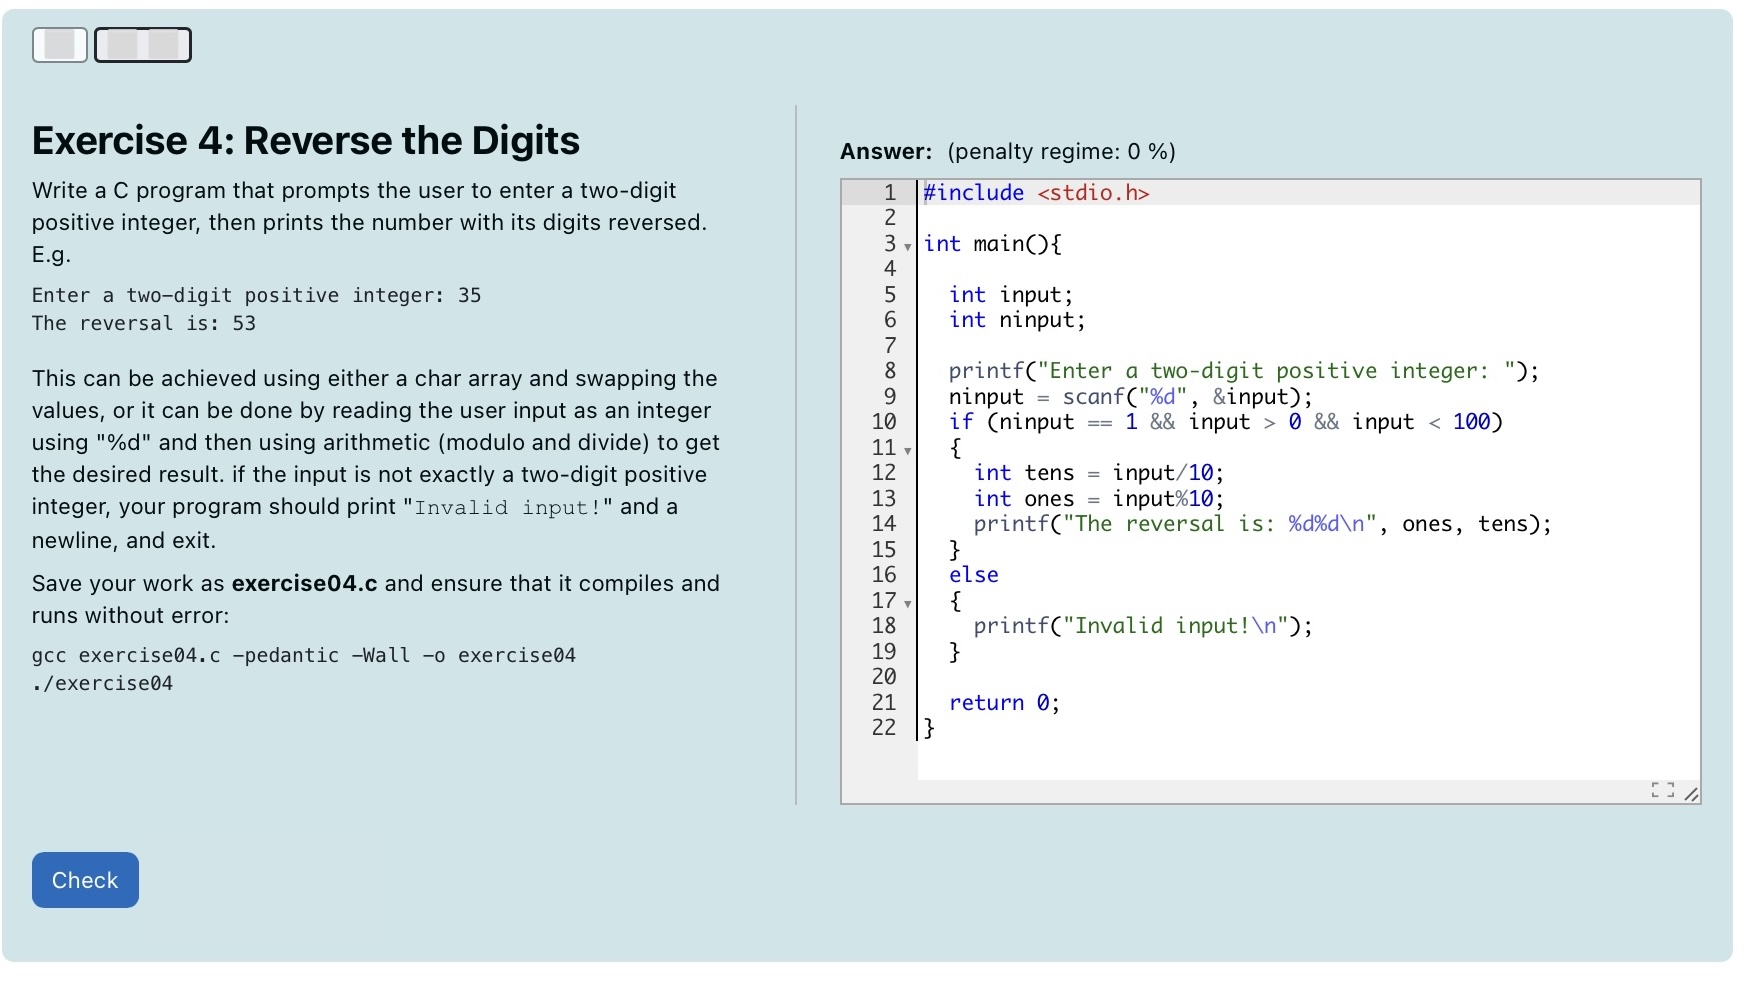
\includegraphics[width=0.72\linewidth]{figs/studentanswer_1.jpg}}
        \caption{Side-by-side view}
        \label{fig:studentanswer_sidebyside}
    \end{subfigure}

    \vspace{1em}
    \begin{subfigure}{\linewidth}
        \centering
        \fbox{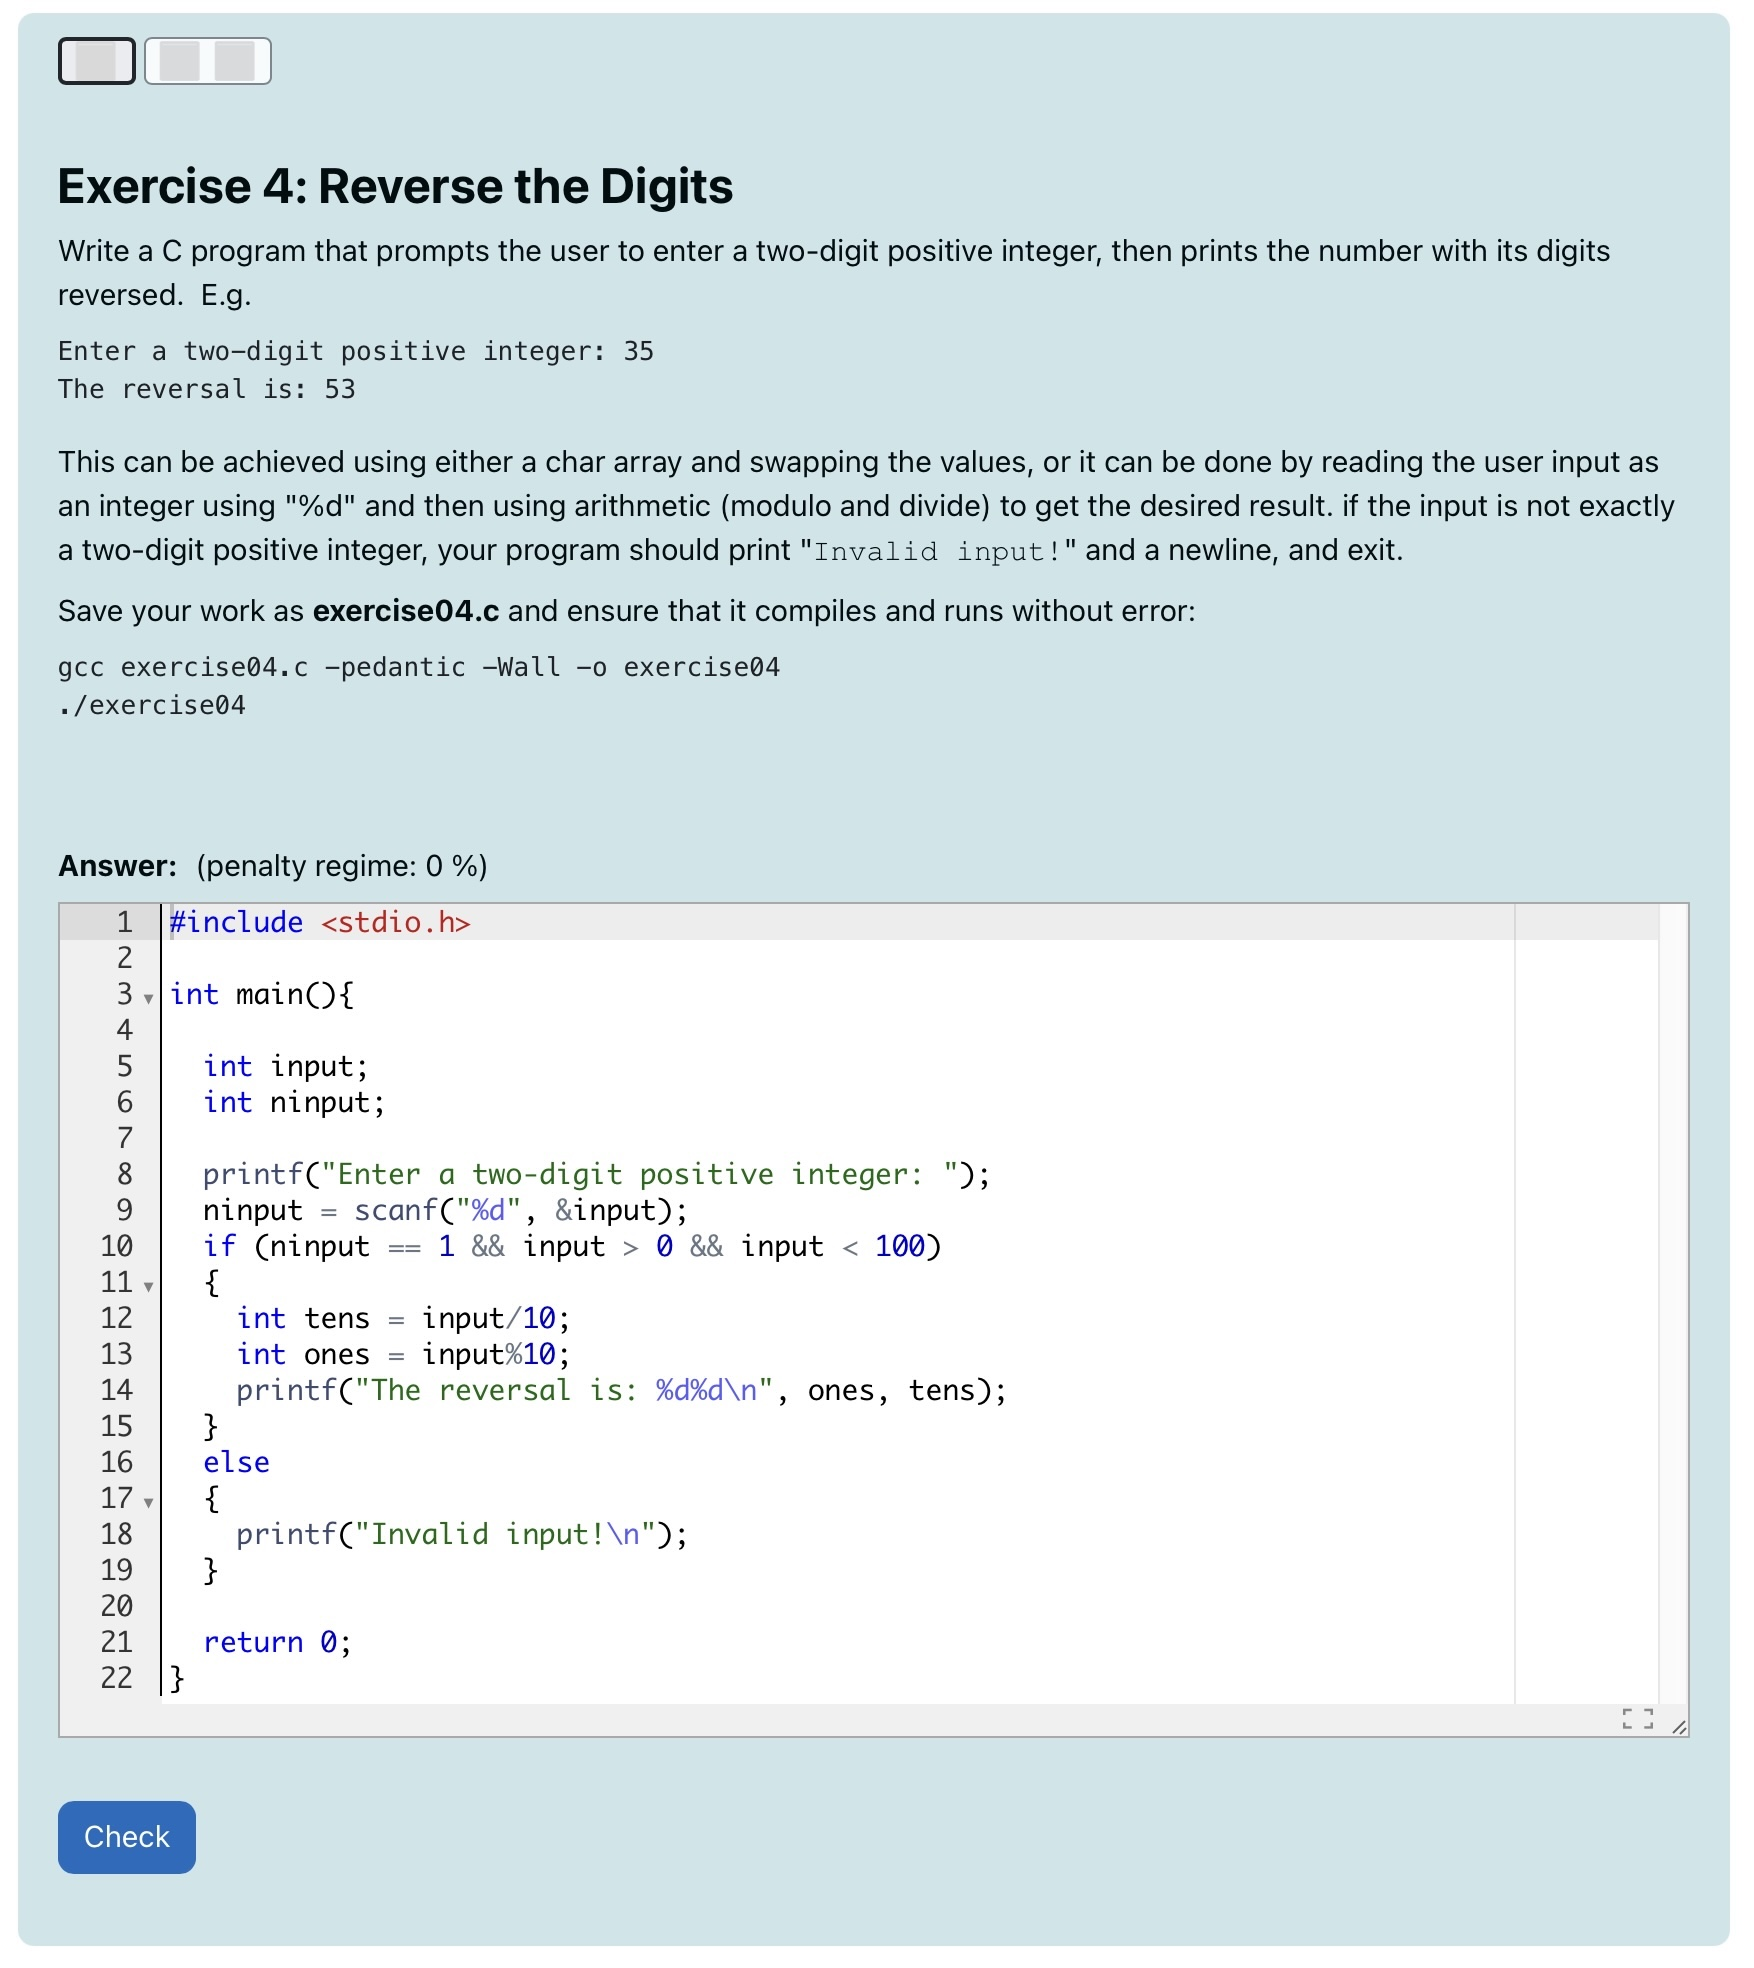
\includegraphics[width=0.6\linewidth]{figs/studentanswer_2.jpg}}
        \caption{Stacked view}
        \label{fig:studentanswer_stacked}
    \end{subfigure}
    \caption{The two student-facing question layouts offered by the layout switcher.}
    \label{fig:studentanswer_layouts}
\end{figure}

The Draft button found on the student-facing page was designed with the Bootstrap CSS framework in mind: Moodle itself uses Bootstrap at its core to style their interface, which allows existing button styles to be reused. With respect to the other existing buttons, the Draft button is styled as the lowest priority, the least attention-grabbing; the gray outlined button is barely noticeable until it is looked for: discoverable but not offensive to the eyes (Figure~\ref{fig:savedraft}).


\begin{figure}[H]
    \centering
    \setlength{\fboxsep}{0pt}%
    \begin{subfigure}[b]{0.48\textwidth}
        \centering
        \fbox{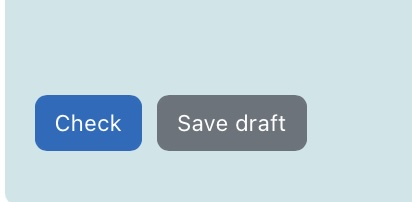
\includegraphics[height=2.5cm]{figs/coderunner-save-draft.jpg}}
        \caption{Hovered view}
        \label{fig:savedraft_hovered}
    \end{subfigure}
    \hfill
    \begin{subfigure}[b]{0.48\textwidth}
        \centering
        \fbox{
\includegraphics[height=2.5cm]{figs/savedraft.jpg}}
        \caption{Unhovered view}
        \label{fig:savedraft_unhovered}
    \end{subfigure}
    \caption{The Save Draft button, hovered and unhovered.}
    \label{fig:savedraft}
\end{figure}

The test cases found on the author page had their styles updated, and a new button was added for deleting test cases. This button also requires the user to confirm their choice using an alert dialog to prevent accidental work loss.

The info panel on the student-facing page was slightly reworked by the addition of a fold/float button. This button was originally designed to completely hide the info panel to allow the page to reduce its margins therefore allow the main content to consume more space for improved readability; however, experimenting with the panel revealed it already supported a different variant of this in the mobile version of the student-facing page. The in-place alternate style is leveraged by allowing the user to use a button to manually set the info panel into mobile mode.

The documentation page added by this project required almost zero interface design because of how the system is designed: the input for this page is entirely Markdown (MD), which lets the PHP MD parser take care of the element and CSS styling. The output is then rendered as HTML onto the page. The input is also a part of the interface because it is written in Markdown, which makes writing up-to-date documentation far more accessible and readable. To quote a survey response: `Currently the best way to learn CodeRunner is to have someone that knows it explain it to you.' Making the documentation accessible and easy to update means that it has the potential to be extended in the future by other contributors and CodeRunner question authors who are experts in it.

\subsubsection{System Design}

The following diagram describes the Docker topology designed for the development part of this project:

\begin{figure}[h]
    \centering
    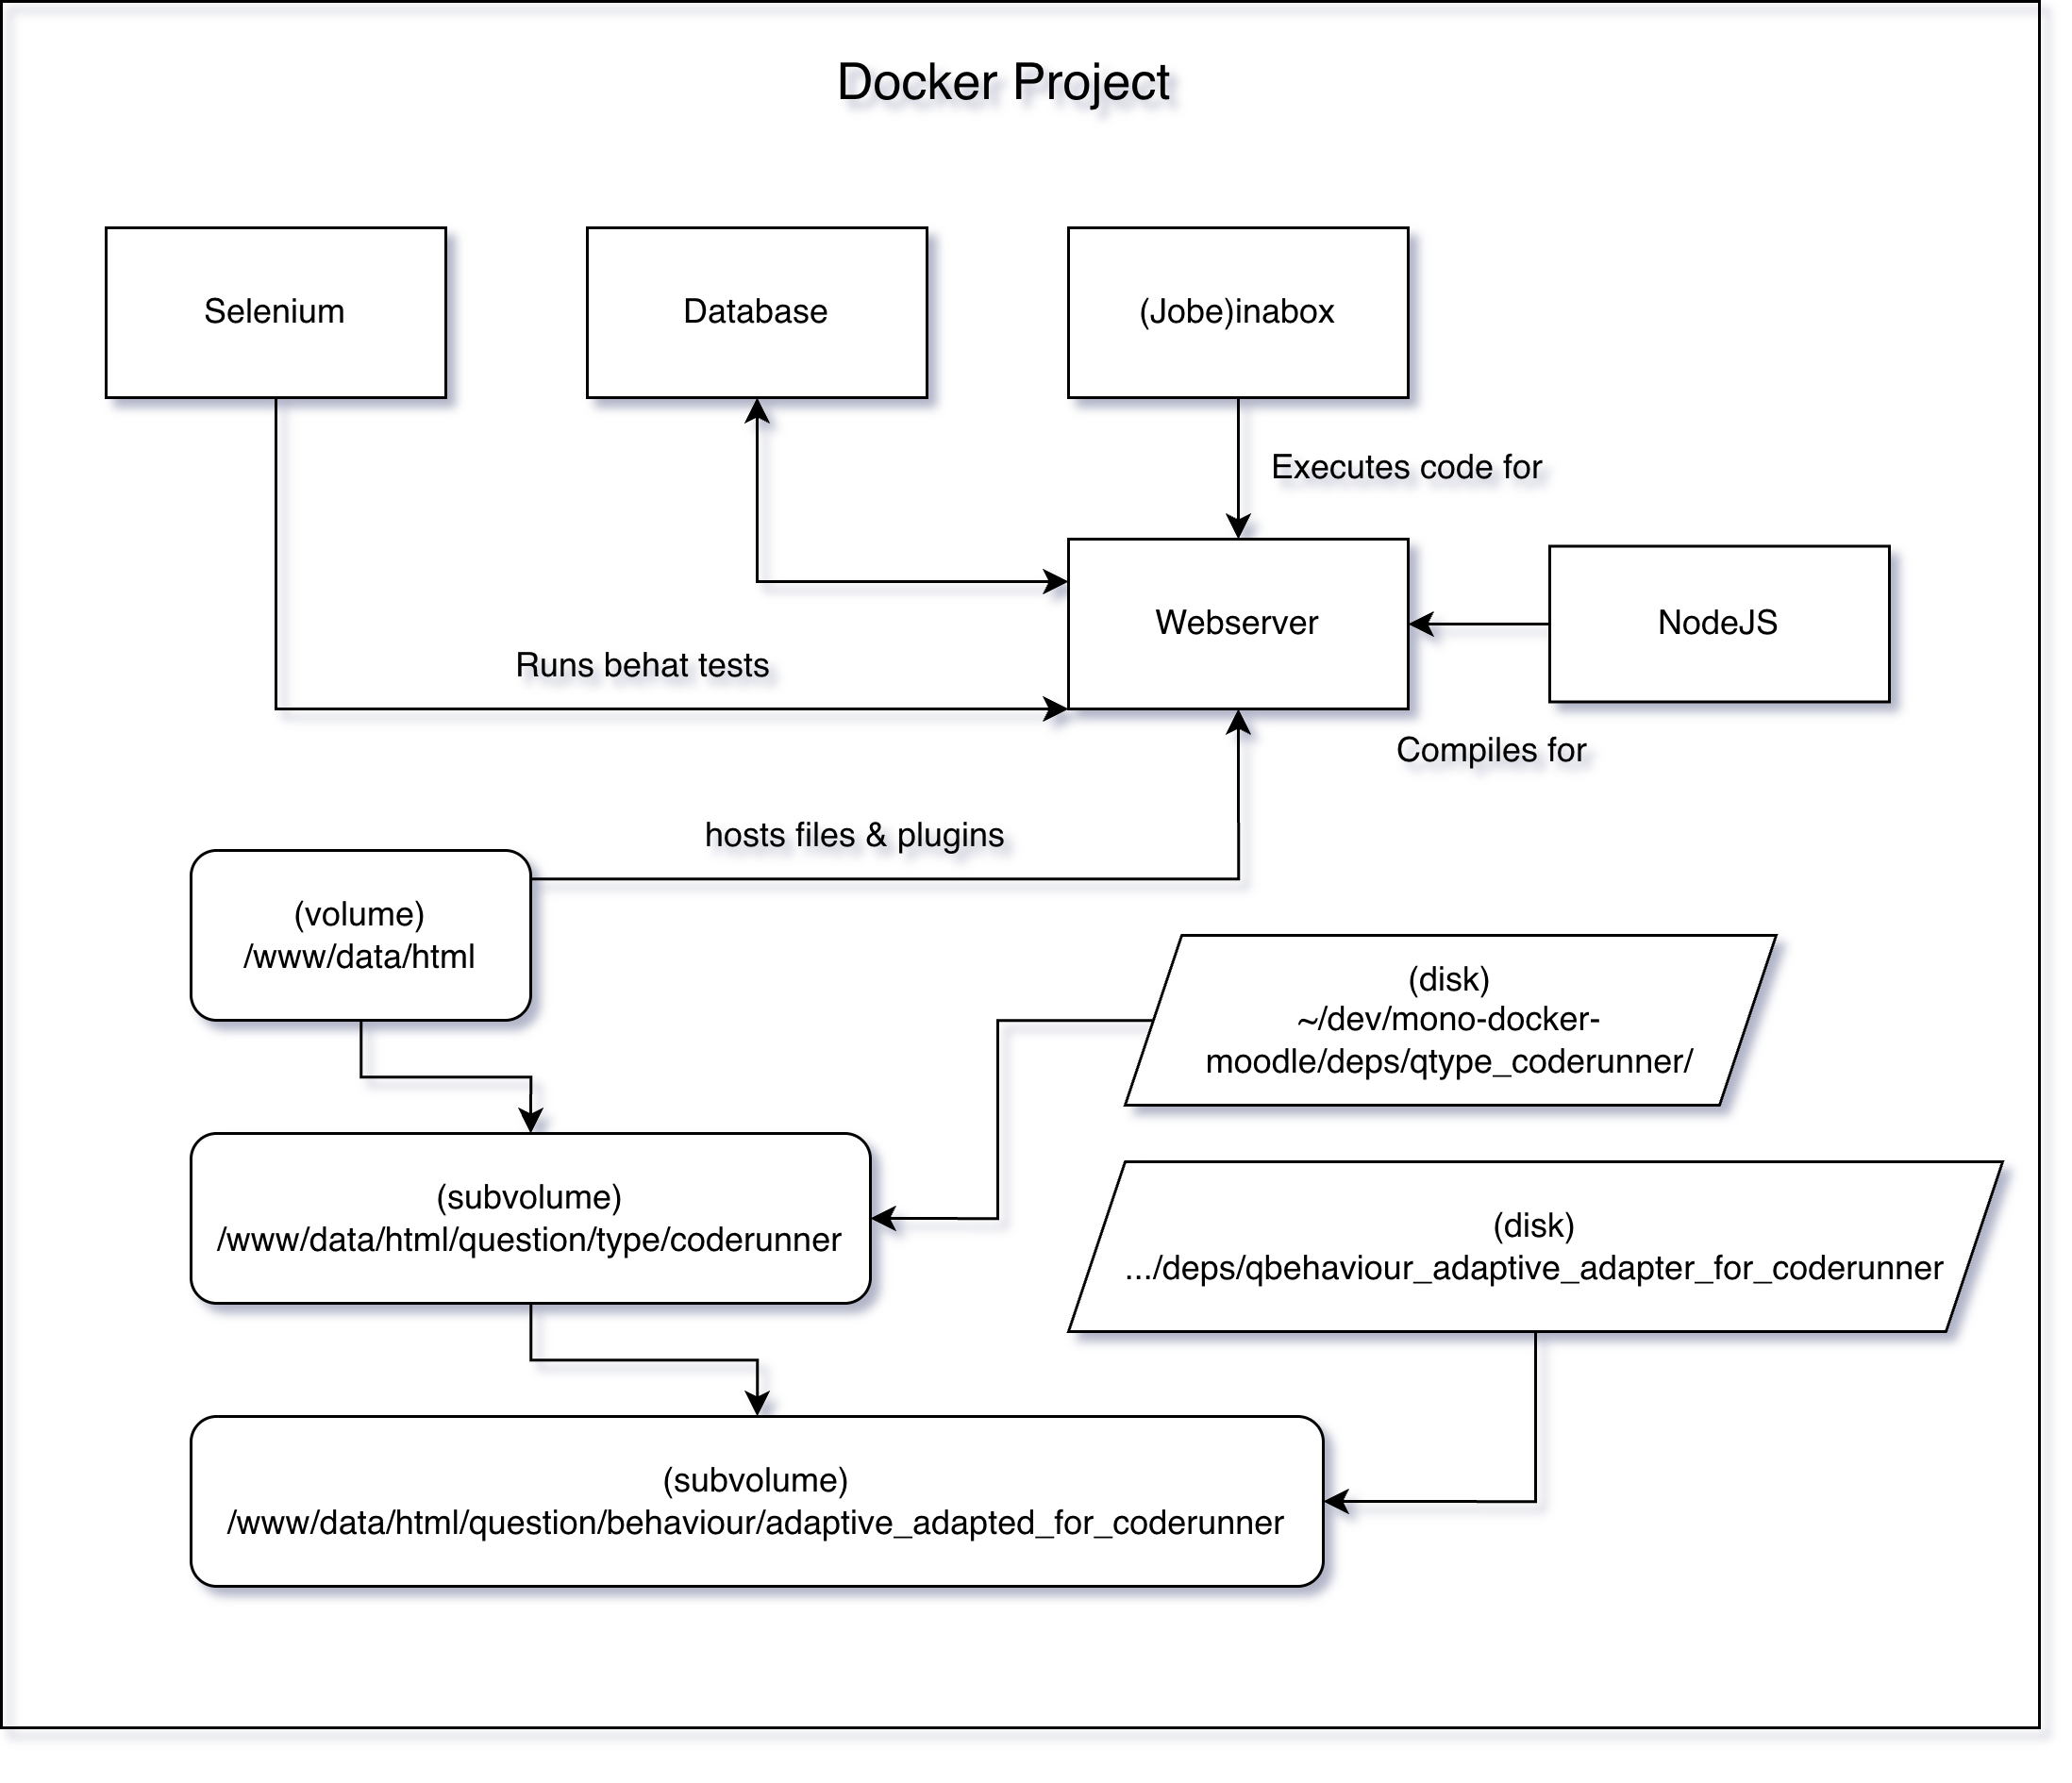
\includegraphics[width=0.8\textwidth]{figs/docker_project.png}
    \caption{Docker architecture}
    \label{fig:docker_project}
\end{figure}

The following diagram is in direct reference to the analysis and describes the sequence of how CodeRunner and Moodle interact to fulfil a question result.

% TODO: insert submission sequence diagram (student -> behaviour plugin -> question type -> Jobe -> result table).

To save the layout state and question info hidden state, a \texttt{sessionStorage} object is used. This allows the page to remember what layout each question was in, sparing the user the cognitive load of recognising what happened to their questions. The data structure avoids polluting \texttt{sessionStorage} with a separate entry per question by keeping all question states under a single key. The data structure in TypeScript goes as follows:
\lstset{
    frame=tb,                           % Frame at top and bottom
    language=Typescript-min,            % Choose the programming language
    basicstyle=\ttfamily\small,         % Use monospace font
    keywordstyle=\color{blue}\bfseries, % Style for language keywords
    commentstyle=\color{green!50!black},% Style for comments
    stringstyle=\color{orange},         % Style for strings
    numbers=left,                       % Line numbers on the left
    numberstyle=\small\color{gray},      % Style for line numbers
    breaklines=true,                    % Wrap long lines automatically
    tabsize=4                           % Set tab spaces
}
\begin{lstlisting}[caption={TypeScript definition for Layout \& Question Info state}]
type QuestionState = {layout: string, infoCollapsed: boolean};
type QuestionID = string;
type QuestionStateTracker = Record<QuestionID, QuestionState>;
// Instead of a new sessionStorage entry per question,
// all question states are stored under one key.

const STORAGE_KEY = 'coderunner_layout';
let state: QuestionStateTracker =
    JSON.parse(sessionStorage.getItem(STORAGE_KEY) || '{}');
let question = state[questionID];
let layout = question.layout;
let infoCollapsed = question.infoCollapsed;

\end{lstlisting}

In some circumstances where the default option is different from the user-chosen option, such as the alternate layout, the page may render with the default option (e.g. style rules), then a lazily loaded script changes it. This sequence happens within 500ms on a good machine, which appears janky and broken. To prevent this, a script was added to the main renderer for CodeRunner which is injected into the page and runs before the first paint, preventing the janky behaviour by overriding the defaults to be the user-chosen ones instead.

The test cases in general required a rework to support deleting test cases. Developing a delete test case button for the author page revealed that test cases were managed and accessed by a continuous index, which broke when deleting test cases in the middle of the array. The parts that interacted with the list of test cases were rewritten to access by key instead of array index. This introduced no regressions according to Behat, PHPUnit and manual testing, and allowed the delete test case button to work correctly.

The lack of a database design is a deliberate decision: \texttt{sessionStorage} was chosen because the changes live in the browser instead of the persistent database. This seemed the most appropriate and least time-costly method. Of all the many changes made, any touching the backend are exclusively stateless or required zero changes in database schema, therefore only browser data needed to be saved. From an end-user's perspective, such a feature would not be expected to save the layout across session resets.

 % Add one file per section.
\clearpage
\section{Product}\label{product}

\subsection{Implementation}

% TODO: opening paragraph -- languages and architecture recap. PHP for the
% Moodle-side changes (editor form, renderers, behaviour, docs page),
% JavaScript as Moodle AMD modules (compiled with Grunt via the NodeJS
% container), CSS for styling, Markdown for documentation content, shell
% scripts for the development workflow. 
The implementation of this project uses PHP for Moodle-side changes, JavaScript for Moodle AMD modules (compiled with Grunt via the NodeJS container), CSS for styling, Markdown for documentation content, shell scripts for development workflow.

\subsubsection{Development Environment}
% TODO: describe the docker-compose stack (webserver, database, Jobeinabox,
% Selenium, NodeJS), the bind mounts injecting both plugins, and the three
% automation scripts: compile-amd-coderunner.sh, phpunit.sh, behat.sh.
The development environment uses Docker~\cite{dockerjournal} (Figure~\ref{fig:docker_project}), which deploys several containers including Selenium for testing and NodeJS for compiling. The environment maintains a virtual volume containing the entirety of Moodle and its files, then Docker mounts the files for CodeRunner and its dependency plugin. The docker environment can be used by executing shell scripts; three scripts were implemented to automate environment-variable assignment and to wrap the otherwise lengthy commands for running the PHPUnit suite, running the Behat suite, and compiling the AMD modules in one go.


\begin{lstlisting}[style=shellcmd]
$ docker volume ls -q --filter "name=moodle-docker" | xargs docker volume rm
\end{lstlisting}

This setup meets \textbf{DE1} because the Docker container is isolated and the data produced within is contained. Deleting the hosted volumes within Docker allows starting over without config file hunting across the host.
\textbf{DE2} is met using a shell script `quick-start.sh` which loads the environment variables required to start and executes the docker-compose bin to init and create the environment.
\textbf{DE3} is fufilled by the Selenium container, the Selenium image loads a headless chrome browser controlled by Behaviour Driven Development tests (BDD)~\cite{northbdd} using Behat.

\subsubsection{Test Case Management}
\textbf{FR1} was met by leveraging an existing capability of Moodle's forms library (formslib). The library's \texttt{repeat\_elements()} helper, which CodeRunner already used to render one group of fields per test case, supports author-facing addition of rows but offers row deletion only as an opt-in: its final parameter nominates a button within each repeated group as that row's delete control. A submit button named \texttt{deletetestcase} was therefore added to the repeated group and its name passed to \texttt{repeat\_elements()}. Moodle registers each \texttt{deletetestcase[i]} as a no-submit button: clicking it reloads the form without validating or saving, and on the rebuild formslib omits the deleted row and records the deletion in a hidden field so that it survives further reloads; the deletion only becomes permanent when the question is saved. The button's visible label is not derived from its name; it is looked up with \texttt{get\_string('deletetestcase', 'qtype\_coderunner')} from the plugin's language file, to which the new strings were added, keeping the label translatable like every other string in the plugin.

To guard against accidental deletion, a small script was attached to each delete button that asks for confirmation via the browser's native dialog. The script does not replace the button's behaviour: it merely intercepts the click and cancels the submission when the author declines, so a confirmed click proceeds exactly as it would have without the script. This makes it a progressive enhancement~\cite{mdnprogressiveenhancement}: were JavaScript unavailable, deletion would still work, just without the prompt.

Finally, the delete button alone was not enough, because CodeRunner accessed test cases by contiguous index, e.g. $[0,1,2,3,4]$. If the author deletes test case 1, the submitted arrays instead have the keys $[0,2,3,4]$, a hole in the sequence. Any loop that assumed a dense range would both read the missing index and silently drop the last row, so every such loop had to change to iterate over the keys actually present. Four places were affected: the form-building loop that attaches help buttons and per-row rules to each test case, the validation of Twig-rendered fields, the validation that counts non-empty tests, and the function that copies test cases from the form into the database on save. The validation of non-empty tests is the most interesting case: the fields \texttt{testcode}, \texttt{stdin} and \texttt{expected} are submitted as three parallel arrays sharing row keys, and the old code walked them with a single counter, assuming they were equal in length with no holes. The new code instead takes the union of the three arrays (PHP's \texttt{+} operator on arrays, which keeps every key appearing in any operand) and iterates over the \texttt{array\_keys()} of the result, so a row is validated if any one of its three fields is present, whatever its key happens to be.

\textbf{FR2} was only partially met, and the compromise was deliberate. Upstream, a new question opens with five blank test cases, and the add button appends three more per click, an amount CodeRunner inherited from a Moodle core constant rather than choosing itself. The core constant was first replaced with plugin-owned ones set to one, which met the requirement exactly: a new question opened with a single blank test case and each click added exactly one more. Once the Behat suite was runnable inside the container, however, this turned out to break several of the upstream acceptance tests, which fill a freshly opened form up to its third test case (\texttt{id\_testcode\_2}) and so assume at least three blanks exist before any button is clicked. Rather than rewriting upstream test fixtures for what is largely a cosmetic gain, both constants were reset to three, the smallest initial count for which the unmodified upstream suite still passes. The result improves on upstream (three initial blanks rather than five) but is not exact; the ideal solution, letting the author choose how many rows each click adds, was judged too low in value relative to its cost in test maintenance and deferred. In practice the gap is also narrowed by FR1: surplus blank rows can now simply be deleted.

\subsubsection{Precheck Rendering Fix}
\textbf{FR4} was met through in-browser analysis followed by a deliberately small fix. When the Precheck option on the author page is set to `Selected', each test case gains an extra div holding its test-type selector, and this div was rendering outside the test case's column flow. Inspecting the live page revealed why: the stylesheet lays each test case row out as a flex container, but the script that shows and hides the selector (necessarily client-side, since the div must react to the Precheck setting without a page reload) re-showed it with an inline \texttt{display: block}. Inline styles override the stylesheet, so every toggle dropped the div out of the flex layout. The fix was a single word in the \texttt{authorform.js} module: re-show the div with \texttt{display: flex} instead. The size of the change is out of all proportion to the analysis required to locate it, which is arguably the mark of a well-aimed fix rather than a small effort.

With the div rendering correctly, one styling wrinkle remained. The selector sat at the bottom of each test case card, where the card's rounded-corner styling belongs to the last visible element, but whether the selector is visible depends on the Precheck setting. That left two options: reorder the form elements so the selector sits in the middle of the card, or dynamically pass the rounded-corner styling between the selector and the element above it as visibility changes. The reorder was chosen, a small server-side change to the form definition, accepting the minor cost that authors accustomed to the old layout must find the selector in its new position; since it moved past only a single element group, that cost is low. The alternative would have tied presentation logic to the Precheck state for a purely cosmetic outcome.

\subsubsection{Save Draft Button}
To meet \textbf{FR6}, a Save draft button was added to the controls beneath the answer box. Previously, a student's only explicit way to save was the Check button (a graded submission that can cost marks under the question's penalty regime~\cite{CodeRunner2016}), so saving work-in-progress meant either paying that penalty or trusting the browser not to lose the page. The new button provides a zero-cost, on-demand persistence point: it stores the current answer and changes nothing about grading. It should be noted that Moodle does periodically (every 60s) automatically save the answer box content. It is, in short, an affordance~\cite{designofeveryday}.

The change is small (28 lines across three files) and lives entirely in the companion behaviour plugin rather than the question type. This placement was deliberate. In Moodle's question architecture~\cite{moodlequestionbehaviours}, the question type defines what a question is, while the behaviour governs how responses are processed; a save control is a submission concern, so it belongs to the behaviour. It also means any question using this behaviour gains the button, and the question type remains presentation-only.

The implementation exposes existing machinery rather than building new. The renderer emits a submit button whose name is generated by \texttt{get\_behaviour\_field\_name('savedraft')}, Moodle's namespacing scheme that routes the click to the correct question's behaviour even when several questions share a quiz page; the construction mirrors the core \texttt{submit\_button} renderer so the button participates in the question engine's usual JavaScript handling, and it is rendered inert on read-only review pages. The behaviour then declares \texttt{savedraft} as expected data, but only while the attempt is unfinished; the engine discards any submitted field a behaviour has not declared, so this single declaration is what makes the button function, and the guard ensures a closed attempt can never be drafted against. Notably, no processing code was required at all: because \texttt{savedraft} is not one of the engine's recognised grading actions, the submission falls through to the engine's default save path, which stores the response as a new step without grading or penalty. The feature's label is resolved from a new language string, keeping it translatable like the rest of the plugin.

On reflection, however, the button worked against its own purpose. Moodle already autosaves the answer box roughly every sixty seconds, so the control added no capability, only interface weight, and the follow-up hint had to be built simply to explain a save that was already happening. A reassurance that must be spelled out by a live, ticking status line ceases to reassure: it draws the eye to the very possibility of loss it was meant to dispel, adding cognitive load in the name of comfort~\cite{dontmakemethink}. A control whose job is to ease concern should not become a source of it, so both the button and the hint were removed. \textbf{FR6} is in consequence met only in part: a student's work is preserved silently by Moodle's periodic autosave, but the explicit on-demand control the requirement named is gone by design. The survey's endorsement of the button is weighed against this decision in the reflection.

\subsubsection{Layout Switcher}
To meet \textbf{FR7}, a per-question layout switcher was built offering two arrangements: the traditional stacked view, and a side-by-side view that places the question text and the answer box in adjacent columns. The server-side renderer was changed to wrap the two halves in dedicated \texttt{question\_box} and \texttt{answer-box} containers (CSS can only arrange what the markup separates), and a new AMD module, \texttt{layoutswitcher.js}, is initialised for each CodeRunner question on the page. The module injects a pair of toggle buttons and implements the modes as a single CSS class toggled on the question's outer div: the JavaScript only flips state, while the layout rules themselves live in the stylesheet.

In the side-by-side mode, a draggable divider separates the two boxes. Dragging recomputes the boxes' widths as ratios, written to their \texttt{flex} properties, so a chosen split survives later window resizes proportionally instead of pinning either side to a pixel width; both sides are clamped to a minimum width (150 pixels, or half the available space when narrower) so neither box can be dragged to nothing or past the other. One subtlety is worth recording: switching modes explicitly clears any inline \texttt{flex} values a previous drag left behind, because inline styles would otherwise override the stylesheet's rules indefinitely, the same class of fault as the Precheck rendering bug above.

The chosen layout persists in \texttt{sessionStorage} under a single key, recorded per question, so two questions on the same quiz page can hold different layouts. The stored entry began life as a bare layout string and later grew into a small object shared with the info panel state of the next section; a migration path still accepts the legacy form. \texttt{sessionStorage} was a deliberate choice: it needs no server round-trip and no database schema change, and it holds nothing personal, only a layout preference keyed by question id, a point the Security section returns to.

Finally, the saved layout is applied before the page paints. Because the AMD module loads asynchronously, a question saved as side-by-side would otherwise render stacked and visibly jump when the module initialised, a layout shift~\cite{webdevcls}: the jank problem discussed in Section~\ref{process}. The renderer therefore emits a small inline script ahead of the question markup that reads \texttt{sessionStorage} and applies the layout class before first paint, eliminating the flash; it is wrapped in a try/catch that falls back to the stacked default wherever \texttt{sessionStorage} is unavailable. Throughout the module, every DOM lookup is guarded, so a question rendered without the expected markup silently receives no controls; and the entire feature is client-side, with no question-processing code touched, so it carries no grading or data-storage risk.

\subsubsection{Info Panel Collapse}
To meet \textbf{FR8}, the student is given a way to reclaim the width that a question page holds in reserve. Two separate things waste horizontal space on a CodeRunner question, and both matter more here than for ordinary question types, because code wants room: Moodle floats a fixed-width info panel (question number, status, marks) beside every question, indenting all of its content; and the Boost theme caps the width of the page content as a whole, leaving dead margins on either side. A small toggle button added to each question's info panel reclaims both at once. Collapsing removes the panel's float, so it stops reserving its column and reflows as an ordinary block while the question content expands beneath it, and simultaneously raises the theme's page-width cap so the whole content area widens into the margins.

The feature went through one design iteration worth recording. The first version hid the panel entirely (shrinking it to the size of the toggle button and hiding its children), which reclaimed the column at the cost of the question number and marks disappearing with it. The final version reflows rather than hides: no information is lost; it merely stops costing a dedicated column. The distinction between removing content and removing the space reserved for content is what the requirement was really asking for.

Two details deserve mention. First, the page-width half of the feature must coordinate across questions: a quiz page can hold several questions, all sharing one page-width cap. The module therefore keeps a page-level set of every question whose panel is currently collapsed; the cap is lifted when the first panel collapses and restored only when the set is empty again, since restoring it any sooner would shrink the page out from under another question still relying on the extra width. Second, the page-level step is deliberately theme-tolerant: it targets a wrapper element specific to Boost-family themes, and on any theme without that markup it is a guarded no-op; the panel itself still collapses normally, so the feature degrades to its within-question half rather than breaking.

The collapsed state persists per question in the same \texttt{sessionStorage} record as the layout choice (this is the change that grew the stored entry from a bare layout string into the small object described in the previous section), and the renderer's pre-paint script applies it before first paint, giving the collapse the same protection against the flash-and-jump behaviour as the layout itself. On narrow (mobile-width) screens the toggle is hidden entirely: the info panel already stacks above the question there, so there is no column to reclaim.

\subsubsection{Accessibility}
To meet \textbf{NFR2}, the author page was audited with Chrome's Lighthouse tool, whose accessibility checks derive from the Web Content Accessibility Guidelines~\cite{w3c_wcag22_2023}, and the findings were worked through. The page initially scored 93\%. The largest issue was that several of the page's selects are rendered by Moodle as grouped controls (the question type, give-up and feedback groups) where the visible label belongs to the group rather than to the select inside it, leaving the selects with no accessible name. This was fixed with \texttt{aria-labelledby} attributes~\cite{w3c_wai_aria12_2023} pointing each select at the id of its group's existing label element. \texttt{aria-labelledby} was chosen over \texttt{aria-label} on purpose: it reuses the visible text instead of duplicating it, so a future edit to the label cannot silently desynchronise the accessible name. This took the audit score to 97\%, and the remaining three percent lies in TinyMCE, Moodle's bundled rich-text editor, which the plugin cannot modify; this measured ceiling is where the requirement's figure of ``97\%, the maximum attainable given third-party components'' comes from.

The new controls this project introduced were held to the same standard. The layout switcher's buttons are icon-only (two squares against one), meaningless to a screen reader, so both carry descriptive \texttt{aria-label}s; the info panel toggle does the same, updating its label to match its state. The same buttons also gained visual contrast: they originally sat at low opacity with pale borders, making the active state nearly indistinguishable, and were reworked with solid backgrounds, darker borders and an unambiguous active style, so state is perceivable without relying on subtle opacity differences.

One piece of accessibility work remains unfinished, and is reported as such. When a student runs their code, the test results should be announced to a screen reader when they arrive; \texttt{aria-live}~\cite{w3c_wai_aria12_2023} was added to the results container and the results message given an addressable id in preparation. It does not yet work, and the cause is known: the results div is replaced wholesale on submission rather than mutated in place, so the live-region registration is destroyed along with the element it was attached to. Fixing this properly means restructuring how the renderer swaps in results, which is scoped as future work.

\subsubsection{Documentation Page}
To meet \textbf{NFR3}, a documentation page was added to the plugin itself. Upstream CodeRunner's documentation lives on an external site, which the editor's help strings link out to; an author who gets stuck mid-task must therefore leave Moodle and search a general-purpose manual. The new page instead serves task-focused documentation from inside the plugin, following the task-oriented, scannable structure recommended for developer documentation~\cite{googledevstyle}: a new script, \texttt{docs.php}, renders Markdown pages within the normal Moodle page chrome, so the documentation is styled and navigated like part of the site the author is already working in.
The page is reachable directly from the question editing form: a ``CodeRunner Documentation'' link, added by \texttt{edit\_coderunner\_form.php} above the form body, opens the index page, so an author never has to leave the task to consult it. This completes the reachability half of NFR3.

The mechanics were chosen for simplicity of authorship. Content is plain Markdown in a directory inside the plugin, rendered with Moodle's bundled MarkdownExtra parser (introducing no new dependency), and the directory is scanned recursively for pages, so adding documentation means adding a file, with no registration step. One rendering defect had to be fixed along the way: MarkdownExtra emits headings without \texttt{id} attributes, so in-page links to sections silently did nothing. A custom \texttt{header\_id\_func} was supplied that slugifies each heading into an anchor id, restoring in-page navigation. This in turn surfaced a PHP 8.1 deprecation notice inside the parser itself, which is silenced narrowly around the single transform call, with a comment recording why and a note to contribute a proper fix upstream.

Because \texttt{docs.php} turns a request parameter into a file path, it is the one place among the project's changes that handles a classically dangerous input, the path traversal weakness~\cite{cwe22}. The parameter is first cleaned by Moodle's \texttt{optional\_param()} with \texttt{PARAM\_PATH}, then resolved with \texttt{realpath()} and required to lie inside the documentation directory; traversal attempts and nonexistent pages alike raise a Moodle exception rather than reaching the filesystem. The script was also written to be testable: it declares its globals explicitly so PHPUnit can include it from within a test, and its unit tests attack exactly this path-containment defence, as the Verification section describes. The content written for the page comprises a revised editor-usage guide and a new question-templating guide.

\subsubsection{Documentation Search}
A scannable page still has to be searched once it grows, and the survey's criticism of the upstream manual as ``monolithic and hard to search'' applies to any single-file documentation. A search facility was therefore added over the same set of pages. Rather than query the server on every keystroke, the design builds an index once and filters it in the browser, which the small corpus makes not merely adequate but preferable. A separate endpoint, \texttt{docs\_searchindex.php}, walks every Markdown page, splits it at its headings, and emits a JSON array in which each section carries its page, anchor, heading and plain text. A lazily loaded AMD module fetches this index the first time the search is opened, caches it, and performs all subsequent matching client-side. The feature postdates the survey and so was not itself evaluated, but it extends the same NFR3 goal the survey endorsed and answers a criticism the survey recorded.

Indexing the pages on the same section boundaries they are rendered with meant the section logic had to be shared rather than duplicated, and this is what motivated extracting the rendering helpers, slugification, transformation and section-wrapping, out of \texttt{docs.php} into the \texttt{lib/docslib.php} library: the rendered page and the search index are now produced from one tested implementation. Matches are ranked so that a whole-phrase hit in a heading outranks one in body text, which in turn outranks scattered single-word hits, and each result is shown with a breadcrumb of its heading path and a snippet in which the matched terms are highlighted. The interface follows the command-palette convention common in developer tools: a bar docked at the top of the page opens, on click or \texttt{Ctrl+K}, into a centred modal over a dimmed backdrop that is navigable entirely by keyboard. The modal is rendered as a fixed overlay attached to the document body so that it floats above the page rather than displacing the content, and it closes on choosing a result, pressing \texttt{Escape} or clicking away. Its index-building and section-wrapping logic is covered by the documentation-library unit tests listed in Appendix~B.

\subsubsection{Security and Personal Data}
No personal data is collected at any point. The survey that informed the requirements was administered through Qualtrics and its responses were anonymous, with any incidental identifying information redacted before analysis (Section~\ref{results}); the software changes themselves gather nothing. The only client-side state introduced is the layout preference, held in the browser's \texttt{sessionStorage} and keyed by question id: it records an interface choice rather than anything about the user, and never leaves the browser. Code execution is unaffected and remains isolated on the Jobe sandbox exactly as upstream.

The changes add only a small attack surface, and every dangerous path is both defended and directly attacked by an automated test rather than assumed safe. The documentation page is the one component that turns a request parameter into a file path, the classic path-traversal weakness~\cite{cwe22}; it cleans the parameter with \texttt{PARAM\_PATH}, resolves it with \texttt{realpath()} and requires the result to lie inside the documentation directory, and its unit tests attack that defence with a request for \texttt{../../version.php}, a real file outside the tree, so a pass means the containment held against a genuine escape rather than a token one. The one-click example importer performs a privileged write, creating questions inside a course, and is guarded by both a capability check and a session-key (CSRF) token; its tests assert that an import is refused when the capability is missing and when the session key is absent, alongside the rejection of malformed slugs. The security-sensitive additions are therefore covered by tests that try to break them, not merely to exercise them, so the guarantees rest on demonstrated behaviour rather than inspection.

\subsection{Verification \& Validation}

\subsubsection{Verification}
Automated verification rests on the two test harnesses of the development environment, each runnable with a single script, and the documentation code is the most heavily tested. Splitting the rendering logic out of \texttt{docs.php} into a library, \texttt{lib/docslib.php}, was done partly to make it unit-testable: nine unit tests exercise the pure helpers directly (heading slugification, Markdown configuration, page discovery, section wrapping, example-list expansion and search-index construction), while seven further tests drive \texttt{docs.php} end to end by faking the request and capturing what it renders. The path-containment defence is attacked rather than merely exercised: the traversal test requests \texttt{../../version.php}, a real file outside the documentation directory, so it cannot be satisfied by a naive existence check. The one-click example importer and the test-case indexing rewrite are covered too, by nine and two tests respectively, the latter confirming that deleting a test case from the middle of the form leaves the survivors correctly paired. In total the project contributes twenty-seven PHPUnit tests, all of which pass; the case-by-case listing is given in Appendix B.

For regression testing, the plugin's upstream Behat suite was run unaltered: browser-driven acceptance tests, executed against the Selenium container by \texttt{behat.sh}. Their evidential value comes from their provenance (tests not written by this project, exercising code it changed), so passing them is independent evidence that the test-case indexing rewrite preserved existing behaviour. The suite also demonstrably earned its keep: it exposed that the one-blank test-case defaults broke upstream scenarios, forcing the reset to three described under FR2, a concrete regression caught by the harness before any user saw it and justification for the effort spent making the suite runnable (DE3). Three further Behat scenarios were written for the project's own features, covering the layout switcher, documentation navigation and the editor's documentation link.

The remaining evidence is measured or manual. Lighthouse audits provide the quantitative check for NFR2, with the before and after scores (93\% and 97\%) recorded at the time of the change. The interactive interface features (the info panel collapse and the precheck fix) were verified manually, both directly and through the closed feedback loop of peers and supervisor described in Section~\ref{process}, with the layout switcher additionally covered by an acceptance test. The limitation is stated plainly: automated coverage concentrates on the documentation, importer and question-type code together with the upstream suite, while the remaining interactive behaviour is checked by acceptance tests and manual review rather than unit tests.

\subsubsection{Validation}
Validation against the requirements is summarised in the traceability table (Table~\ref{tab:traceability})~\cite{goteltraceability}, which traces each requirement from Section~\ref{process} to its implementation, the evidence that verified it, and its status. The statuses are kept honest rather than uniform: most requirements are met, FR2 and FR6 are met partially (the trade-offs are argued in their respective implementation sections above), and three were deferred.

The deferred requirements were scoped out deliberately rather than silently dropped, and were the lowest-priority (\emph{Could}) items in the specification. FR5 (hints for hidden test cases) and FR9 (a copy button on code blocks) both originated in the user survey, and neither is abandoned: the Results section reframes the hint mechanism as the broader question of how much information hidden test cases should reveal, and identifies the copy button as future work with a high benefit-to-cost ratio. FR3 (keeping help content visible until the author dismisses it) was deferred on the same basis, a lower-priority refinement to the author form left for future work. Deferring all three was a scoping decision made against the time remaining.

\begin{table}[h]
\centering
\small
\renewcommand{\arraystretch}{1.2}
\setlength{\abovecaptionskip}{0pt}
\setlength{\belowcaptionskip}{12pt}
\caption{Requirements traceability: each requirement from Section~\ref{process}, its implementation, and its verification evidence.}
\label{tab:traceability}
\begin{tabular}{@{}l p{0.30\linewidth} p{0.22\linewidth} p{0.14\linewidth} l@{}}
\toprule
\textbf{ID} & \textbf{Requirement} & \textbf{Implementation} & \textbf{Verified by} & \textbf{Status} \\
\midrule
\multicolumn{5}{@{}l}{\textit{Development environment}} \\
\addlinespace[2pt]
DE1 & Environment isolated from host & Docker compose stack & Manual & \statusmet \\
DE2 & Single command, repeatable setup & quick-start / compose scripts & Manual & \statusmet \\
DE3 & Regression testable & phpunit.sh, behat.sh & PHPUnit, Behat & \statusmet \\
\addlinespace
\multicolumn{5}{@{}l}{\textit{Functional requirements}} \\
\addlinespace[2pt]
FR1 & Delete test cases & repeat\_elements delete button & Behat, manual & \statusmet \\
FR2 & Add exact number of test cases & NUM\_TESTCASES 3/3 & Behat, manual & \statuspartial \\
FR3 & Help content stays visible & Not implemented & -- & \statusdeferred \\
FR4 & Precheck renders in correct column & authorform.js fix & Manual & \statusmet \\
FR5 & Hints for hidden test cases & Not implemented & -- & \statusdeferred \\
FR6 & Save work on demand & Moodle periodic autosave & Manual & \statuspartial \\
FR7 & Manage question layout & Layout switcher & Manual & \statusmet \\
FR8 & Reclaim margin space & Info panel collapse & Manual & \statusmet \\
FR9 & Copy button on code blocks & Not implemented & -- & \statusdeferred \\
\addlinespace
\multicolumn{5}{@{}l}{\textit{Non-functional requirements}} \\
\addlinespace[2pt]
NFR1 & Visual consistency & styles.css rework & Peer review & \statusmet \\
NFR2 & Lighthouse accessibility $\geq$ 97\% & ARIA labels & Lighthouse audit & \statusmet \\
NFR3 & Effective, reachable documentation & docs.php + content & PHPUnit, survey & \statusmet \\
\bottomrule
\end{tabular}
\end{table}
 % Add one file per section.
\clearpage

\section{Results \& Evaluation}\label{results}


\subsection{Evaluation Process}

During the iterative process of designing the interfaces, before they were finalised, the project supervisor helped make styling decisions.

In order to correctly evaluate the interface design, a survey was performed on participants specifically from University of Strathclyde in the Computer Science department. The demographic ranged from Students to Lecturers. No other personal information was collected and any personally identifiable information was redacted.
% TODO: this paragraph previously ended mid-sentence ("Furthermore,") --
% restore the intended continuation if one was planned.

The survey as of \emph{18 July 2026} settled on 24 participants.

Unfortunately, a functional assessment where end-users tangibly interact with the interfaces was not possible due to time constraints and issues surrounding what happens with the data collected such as GDPR and user consent. The data would be stored on personal drives, which would define the surveyor as liable. 

It was decided it was best to use Qualtrics instead, where the survey contained 8 questions, varying by 2 less if you selected to be declare yourself a student. The removed questions were pertaining to the documentation requirement of this project, which meant they were not applicable to students.

\subsection{Results of Evaluation}
This Section includes a direct interpretation of the gathered data and evaluation processes. Figures~\ref{fig:survey_q1}, \ref{fig:survey_q3} and \ref{fig:survey_q5} summarise the responses to the three interface features shown to participants, with each question broken down by respondent type.

\begin{figure}[H]
    \centering
    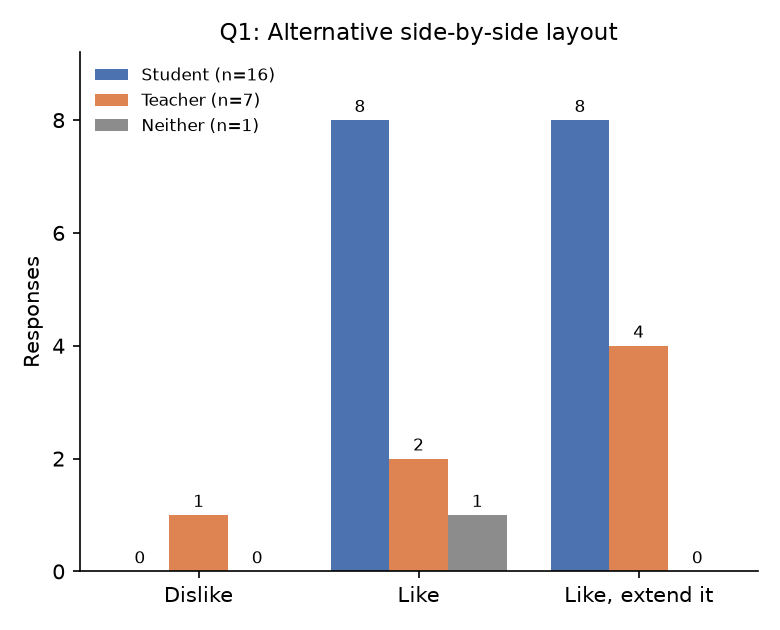
\includegraphics[width=0.7\textwidth]{figs/survey_q1.png}
    \caption{Survey responses to the alternative layout (Q1), broken down by respondent type.}
    \label{fig:survey_q1}
\end{figure}

\begin{figure}[H]
    \centering
    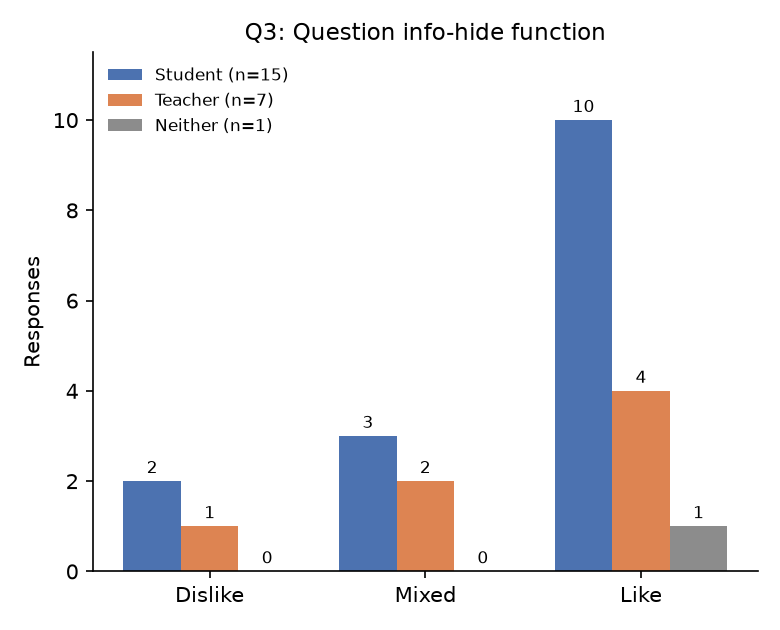
\includegraphics[width=0.7\textwidth]{figs/survey_q3.png}
    \caption{Survey responses to the info-hide function (Q3), broken down by respondent type.}
    \label{fig:survey_q3}
\end{figure}

\begin{figure}[H]
    \centering
    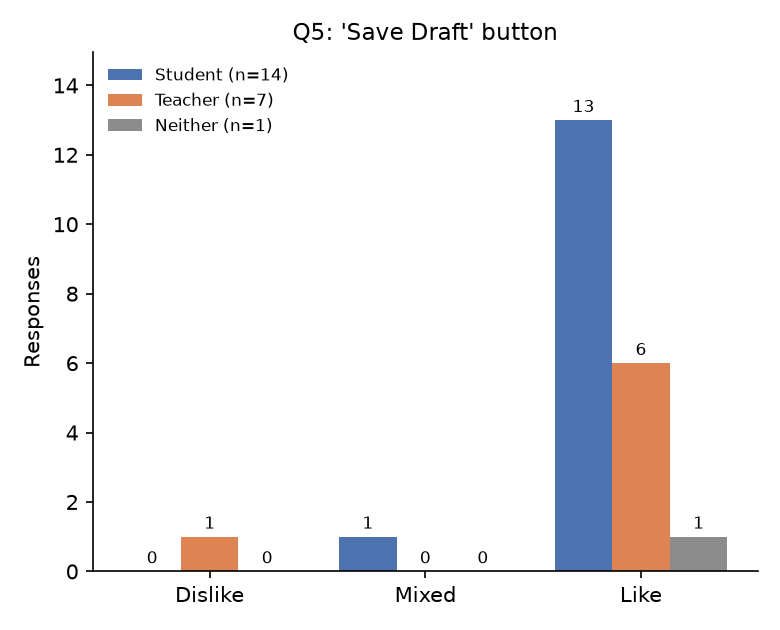
\includegraphics[width=0.7\textwidth]{figs/survey_q5.png}
    \caption{Survey responses to the Save Draft button (Q5), broken down by respondent type.}
    \label{fig:survey_q5}
\end{figure}

\subsubsection{Reception of the Interface Changes}

Reception of the three interface changes was strongly positive across both roles. The alternative side-by-side layout (Figure~\ref{fig:survey_q1}) received the broadest approval: of the 24 responses to the question, 23 (96\%) were positive, and exactly half of all respondents chose the stronger option of liking it and wanting it implemented on other question types. That second figure is notable because it asks for more than FR7 ever specified; extending the layout switcher beyond CodeRunner questions is therefore recorded as future work. The single negative response came from a teacher.

The info-hide function (Figure~\ref{fig:survey_q3}) was the most divided of the three: 15 of 23 responses (65\%) liked it as delivered, 5 (22\%) judged it a good idea if improved, and 3 (13\%) disliked it. This spread is consistent with the feature being the most novel of the three, since it changes how the page itself behaves rather than adding a discrete control. A majority of both students and teachers still approved, and the appetite for refinement points to polishing the interaction rather than removing it.

The Save Draft button (Figure~\ref{fig:survey_q5}) drew the highest approval rate: 20 of 22 responses (91\%) liked it outright, with one response in each of the remaining categories. The result is striking for a control that was styled to be deliberately unobtrusive, and it confirms that students value reassurance that their work is safe. That the button was afterwards removed does not diminish this finding: the approval attaches to the reassurance, not to the button, and the reassurance is better delivered silently by Moodle's own autosave than by a control that had come to demand explanation and attention of its own. The reasoning behind the reversal is set out in the reflection.

Taken together, the survey substantiates the claim that the features it evaluated were worth building: every feature achieved majority approval within both the student and the teacher group, and no feature was rejected by either group.

\subsubsection{Documentation Findings}

The two documentation questions were shown only to non-student respondents, as they concern authoring rather than answering. Seven teachers responded; five of the answers were substantive, and two were test entries which are excluded from the analysis.

On the current state of CodeRunner's documentation, the responses corroborate the assessment made in Section~\ref{process}. Its quality was acknowledged while its form was criticised: `good, but monolithic and hard to search' and `okay, but not always the easiest to understand'. Two responses located the working knowledge outside the manual altogether, one noting that `a lot of the useful stuff is within the forums and needs a bit of searching to find', and another reporting that they had not consulted the documentation since 2021, preferring to work from third-party examples. One respondent summarised the problem in the words quoted in the Design section: the best way to learn CodeRunner today is to have someone who already knows it explain it.

On the proposed alternative, documentation organised around the author form with contextual explanations, four of the five substantive responses were supportive, ranging from `sounds good' to `plenty of other areas use a similar approach so it seems like a no-brainer' and `this would be useful to stop you needing to look it up'. The remaining response raised a considered governance concern rather than an objection: if authors can contribute to the documentation, someone must hold authority over debatable contributions, and clarity should be valued above concision. These points target the future contribution model rather than the documentation page delivered by this project, and they are recorded as considerations for any community-editable extension of it.

These findings validate the direction taken for NFR3: the criticisms of the existing manual match the deficiencies identified in the analysis, and the approach built in response was endorsed by four of the five substantive teacher responses.

\subsubsection{Evaluation Against the Objectives}
The survey speaks directly to the three interface changes it showed, but the project's objectives are broader, and each carries its own evidence. Objective~1, a reproducible, regression-testable environment, is demonstrated by the two single-command test harnesses and the upstream Behat suite they run (DE1--DE3). Objective~2, the author-page ergonomics, combines the survey's endorsement of the layout and information-panel behaviour with the Behat and manual verification of test-case management (FR1) and the Precheck fix (FR4), and with the measured accessibility gain from 93\% to 97\% (NFR2). Objective~3, the student experience, is precisely what the survey assessed: the alternative layout and the info-hide function each won majority approval in both respondent groups, as did the save-draft button that was subsequently removed for the reasons set out in the reflection. Objective~4, task-focused documentation reachable from the tool, is supported by the four of five substantive teacher responses endorsing the approach and by the delivered page, its editing-form link and its search. Objective~5, evaluating the changes with real users to derive further requirements, is discharged by the survey itself, which both validated the delivered work and produced the future-work items discussed in the reflection that follows. The three deferred requirements (FR3, FR5 and FR9) leave acknowledged gaps within the second and third objectives, but no objective is left unmet and no delivered feature was judged unwanted by either audience.

 
\clearpage
\section{Discussion \& Reflection}

\subsection{Interpreting the Results}

The survey results support the project's central bet: that a mature assessment tool's remaining problems are experience problems, not capability problems. All three interface changes achieved majority approval in every respondent group, and the strongest demand recorded was not for something new but for more of the same, with half of all respondents asking for the layout switcher to be extended to other question types. The most divided reception, for the info-hide function, belongs to the change that alters how the page itself behaves rather than adding a visible control; this suggests that features which move existing content need more explanation, or gentler defaults, than features which add something clearly optional.

The documentation findings carry a wider implication. The teachers surveyed did not criticise the quality of CodeRunner's manual, only its shape, and two of them reported working from forums and third-party examples rather than the documentation at all. This matches the analysis in Section~\ref{process} and suggests the real competition for official documentation is not better official documentation but informal knowledge scattered across colleagues and forums. Documentation that lives where the work happens, as built for NFR3, is an attempt to bring that knowledge back into the tool. The one governance concern raised, about who arbitrates contributions, is the correct next question and is addressed under future work.

\subsection{Reflection}

The clearest lesson is written in the project's own commit history: the test environment should have been completed before feature work began, not alongside it. The first behaviour-changing commit was made on 1 July and, among other things, reduced the number of blank test cases a new question opens with. The scripts that make the regression suites runnable only landed on 8 and 10 July, and the Selenium configuration that let the browser tests run reliably was fixed on 17 July. The first full run of the suite that day exposed that the 1 July change had been breaking upstream acceptance tests for over two weeks, and the fix was committed within hours of the harness working. Had DE3 been discharged first, a sixteen-day-old latent regression would instead have been a same-day correction. The requirement was identified early; its priority was misjudged.

A second lesson concerns commit discipline. Several commits bundle unrelated changes, such as accessibility labels arriving in the same commit as the new documentation page, or the test case index rewrite sharing a commit with the delete button and a form reordering. This cost nothing at the time but made later work harder: writing this report, tracing when a regression entered, and understanding which change caused which effect all required untangling commits that should have been three commits each.

Finally, the history records a misjudgement about what counts as work. The commit message for the Precheck rendering fix reads `this is probably the one legitimate fix I've made so far', written after hours of diagnosis produced a one-word change. With hindsight this undervalues exactly the work that mattered: the diagnosis was the fix, and the polish, styling and interface changes dismissed in that message were the substance of the project's requirements. Recognising analysis and refinement as legitimate engineering, rather than only new code, is a perspective this project taught.

A last reflection concerns the Save Draft button, the best-received of the surveyed changes at 91\% approval, which was nonetheless removed from the final plugin. The button was always a small addition of interface weight, justified on the grounds that it reassured students their work was safe. The follow-up auto-save hint was an attempt to make that reassurance explicit, but building it exposed the flaw in the whole idea. Moodle already autosaves the answer box roughly every sixty seconds, so the button added no capability; and a reassurance that has to be spelled out by a live, ticking status line stops reassuring and starts to worry, drawing a student's attention to the loss it was meant to make them forget. A control whose purpose is to ease concern cannot be allowed to add cognitive load or to become a source of concern itself. Removing both the button and the hint, despite the survey's endorsement, was therefore the consistent choice: the approval confirms that students want to feel their work is safe, not that they want a button, and that feeling is best served by the platform saving silently in the background. The wider lesson is to separate a validated need from the particular control that first surfaced it, and to be willing to retire even a popular control when meeting the need better means removing it.

\subsection{Challenges}

The environment consumed far more of the schedule than anticipated. Before any feature could be attempted, the project had to assemble four codebases into one repository, learn Docker from scratch, and diagnose two failures in sequence: macOS permissions silently breaking the shared plugin folders, which forced a switch to a Linux machine, and Moodle's security policy blocking the internal web requests its own components use, which cost many hours because the failure gave no useful signal. The lesson carried forward is that platform security policies should be the first suspect when two locally-run services refuse to talk.

The second sustained challenge was working inside a large, unfamiliar, live codebase. CodeRunner and Moodle's question framework are mature systems with their own idioms, and several tasks that appeared small required understanding those idioms first: the delete button was one parameter, but making it safe required discovering that the form library re-applies help buttons by row index and rewriting every loop that assumed test case indices were contiguous. Estimating work by the size of the visible change proved consistently misleading.

\subsection{Limitations}

The evaluation has clear limits. The survey settled on 24 participants, of whom only seven were teachers, and the documentation questions were shown to teachers alone, leaving five substantive responses after two test entries were excluded; conclusions drawn from that subset are indicative rather than firm. Participants judged the features from images and recordings rather than hands-on use, a constraint accepted for data protection reasons, so the results measure first impressions rather than lived usage. On the product side, the interactive interface behaviour is covered by acceptance tests and manual review rather than unit tests, and three requirements (FR3, FR5 and FR9) were deferred.

\subsection{Future Work}

The survey and the analysis point in the same direction for what to build next. The highest-value item is hints for hidden test cases (the deferred FR5): it was requested in the survey, it addresses the student-side pain the analysis rated most serious, and the literature identifies feedback quality as the field's persistent weakness~\cite{keuningfeedback}. The copy button on code blocks (FR9) remains a small, high benefit-to-cost addition. Beyond the deferred requirements, three items emerged during the project: extending the layout switcher to other question types, which half of all survey respondents requested (however prompted); completing the screen reader announcement of test results, for which the groundwork is in place but the renderer must be restructured to mutate rather than replace its results container; and defining a moderated contribution model for the documentation page, answering the governance concern raised in the survey, so that experienced question authors can extend it without disputes over content. Finally, the changes themselves are candidates for contribution upstream to the CodeRunner project, which would expose them to a far larger user base and subject them to review by the tool's maintainers. 
 
\clearpage
\section{Conclusion}\label{conc}

This project set out to remove the experience-level friction from a capable but ageing assessment tool, and to do so on the live system rather than by replacing it. Each of the five objectives was met. A reproducible Docker environment now rebuilds Moodle, CodeRunner and its dependencies with a single command and runs both test harnesses, providing the regression safety net the rest of the work depended on. The author page gained flexible test-case management and a corrected Precheck display, together with the visual and accessibility improvements the analysis called for. The student page gained a switchable, resizable layout and reclaimable working space. Task-focused documentation, searchable and reachable from the editing form, was served from inside the plugin. The delivered changes were then evaluated with real students and teachers, whose feedback both validated the work and generated further requirements.

The evidence supports the project's central claim: the friction that remains in a mature tool of this kind is a software problem, and disciplined user-experience engineering resolves it. Every delivered feature won majority approval from both audiences, none was rejected, the accessibility score improved, and an independent regression suite showed that nothing already working was broken. Three requirements were deferred, each recorded as future work rather than abandoned. The clearest recommendation that follows is to offer the changes upstream to the CodeRunner project, so that a far larger community of authors and students benefits from them and subjects them to wider review, and to continue the evidence-led approach for the feedback and hint features that users asked for most.




%--------------------------------
% Bibliography
%--------------------------------
\clearpage
\setstretch{1.0}  % 1.0 line spacing. 
\bibliographystyle{abbrv}
\bibliography{bibliography}
% add references to the file called bibliography.bib
\clearpage

%--------------------------------
% Appendices
%--------------------------------
\appendix
\setstretch{1.5} % 1.5 line spacing.
\section{Appendix}

\subsection{Appendix A: Detailed Specification and Design}

\subsubsection{Requirements Specification}

This section restates the requirements introduced in Section~\ref{process} in full, with the source each was elicited from and a MoSCoW priority. Priorities were assigned against the time available: the development environment and the correctness-level author-page defects are treated as \emph{Must}, the interface improvements as \emph{Should}, and the two survey-sourced additions that were ultimately scoped out as \emph{Could}. The status of each requirement and the evidence that verified it are given separately in the traceability table (Table~\ref{tab:traceability}) so that specification and outcome are not conflated.

\begin{table}[h]
\centering
\small
\renewcommand{\arraystretch}{1.2}
\begin{tabular}{@{}l p{0.56\linewidth} l l@{}}
\toprule
\textbf{ID} & \textbf{Requirement} & \textbf{Source} & \textbf{Priority} \\
\midrule
\multicolumn{4}{@{}l}{\textit{Development environment}} \\
\addlinespace[2pt]
DE1 & Run Moodle, CodeRunner and its dependencies in isolation from the host. & Analysis & Must \\
DE2 & Start with a single command and produce a repeatable setup. & Analysis & Must \\
DE3 & Allow CodeRunner to be tested for regressions. & Analysis & Must \\
\addlinespace
\multicolumn{4}{@{}l}{\textit{Functional requirements}} \\
\addlinespace[2pt]
FR1 & Allow the author to delete test cases. & Analysis & Must \\
FR2 & Allow the author to add exactly the number of test cases wanted. & Analysis & Should \\
FR3 & Keep help content visible until the author dismisses it. & Analysis & Could \\
FR4 & Render the Precheck option in its correct column, attached to its test case. & Analysis & Must \\
FR5 & Provide an option to give hints for hidden test cases. & Survey & Could \\
FR6 & Allow the student to save their current work on demand. & Analysis & Should \\
FR7 & Allow the student to manage the layout of the question. & GitHub Issue & Should \\
FR8 & Allow the student to reclaim unused margin space to enlarge the content area. & Analysis & Should \\
FR9 & Provide a copy button on code blocks within the question text. & Survey & Could \\
\addlinespace
\multicolumn{4}{@{}l}{\textit{Non-functional requirements}} \\
\addlinespace[2pt]
NFR1 & Be visually consistent: uniform corner rounding, labels and checkboxes aligned with their controls. & Analysis & Must \\
NFR2 & Score at least 97\% on a Lighthouse accessibility audit. & Analysis & Must \\
NFR3 & Provide documentation that is effective, task-focused and reachable from the question editing form. & Analysis & Must \\
\bottomrule
\end{tabular}
\caption{Requirements specification with elicitation source and MoSCoW priority. Status and verification evidence are in Table~\ref{tab:traceability}.}
\label{tab:requirements-spec}
\end{table}

\subsubsection{System Design}

The system is layered so that the work of this project stays isolated from the platform it extends. At the base is a containerised development environment (Figure~\ref{fig:docker_project}): Docker Compose brings up Moodle on a web-server container, a PostgreSQL database, a JobeInABox sandbox for code execution, a Selenium container for browser tests and a Node container for compiling front-end assets. Moodle and its files live in a managed volume, while the two plugins developed here, the CodeRunner question type and its adapted behaviour dependency, are bind-mounted into that volume from the repository. This arrangement satisfies DE1 and DE2 and means every change is exercised against a real Moodle rather than a mock.

The documentation subsystem was designed for simplicity of authorship and for testability. Content is plain Markdown files under \texttt{docs/editor/}, discovered recursively at request time, so publishing a page requires only adding a file. Rendering is a short pipeline: the raw Markdown is first scanned for an example-list placeholder, which is expanded into per-example import links; it is then transformed to HTML by Moodle's bundled MarkdownExtra parser, configured with a custom \texttt{header\_id\_func} that slugifies each heading into a stable anchor; finally the flat HTML is post-processed to wrap each heading and the content beneath it, up to the next heading, in an anchored \texttt{doc-section} container. Wrapping at this last stage, after transformation, avoids interfering with MarkdownExtra's own block handling. These stages were deliberately extracted from the request script into a library, \texttt{lib/docslib.php}, so that each is a pure function unit-testable in isolation. The page is reachable directly from the question editing form: a documentation link is injected by \texttt{edit\_coderunner\_form.php} above the form body, pointing at the index page, which satisfies the reachability half of NFR3.

The in-plugin search is built on the same section structure. A separate endpoint, \texttt{docs\_searchindex.php}, walks every page and emits a JSON index of sections, each carrying its page, anchor, heading and plain text. The client module, loaded lazily only when the search is first used, fetches this index once and filters it entirely in the browser, which is ample for the small corpus. Ranking favours a whole-phrase match in a heading over one in body text over loose per-word hits, and each result is shown with a breadcrumb of its heading path and a highlighted snippet. The interface is a command palette: a docked bar that opens into a centred modal over a dimmed backdrop, portalled to the document body so that its fixed positioning is measured against the viewport rather than any transformed page wrapper.

Client-side preferences follow a minimal-state design. The layout switcher persists its chosen layout in the browser's \texttt{sessionStorage}, keyed by question id, so a choice survives navigation within a session without being written to the server or tied to the user's identity. No personal data is introduced by any of these changes, and code execution remains isolated on the Jobe sandbox.

\subsection{Appendix B: Detailed Test Strategy and Test Cases}

Testing followed a two-layer strategy. Fast, deterministic PHPUnit tests cover the code this project authored, and the plugin's own browser-driven Behat suite is run unaltered as a regression check on the code the project changed. The extraction of the documentation helpers into \texttt{lib/docslib.php} was undertaken partly to make them unit-testable in isolation, so that the pure logic could be asserted directly rather than only through a rendered page. Security-sensitive input handling is attacked rather than merely exercised: the path-traversal test targets \texttt{../../version.php}, a real file outside the documentation tree, so it cannot be satisfied by a naive existence check. In total the project contributes twenty-seven PHPUnit tests across four files and three Behat scenarios of its own. Every test written for this project passes.

\begin{table}[h]
\centering
\small
\begin{tabular}{@{}p{0.82\linewidth} l@{}}
\toprule
\textbf{Property verified} & \textbf{Result} \\
\midrule
Heading slugification handles spaces, punctuation, casing and empty input & Pass \\
The configured parser is MarkdownExtra and emits \texttt{id} attributes on headings & Pass \\
The documentation directory resolves correctly and contains the index page & Pass \\
Page discovery strips the \texttt{.md} suffix, lists known pages and returns them sorted & Pass \\
Markdown transforms to HTML with anchored headings & Pass \\
Each heading and its body are wrapped in an anchored \texttt{doc-section} container & Pass \\
Content before the first heading is left outside any section & Pass \\
The example-list placeholder expands into per-example import links & Pass \\
Search-index entries carry the page, anchor, heading and text fields & Pass \\
\bottomrule
\end{tabular}
\caption{Unit tests for the documentation library (\texttt{docslib\_test.php}, 9 tests).}
\label{tab:tests-docslib}
\end{table}

\begin{table}[h]
\centering
\small
\begin{tabular}{@{}p{0.82\linewidth} l@{}}
\toprule
\textbf{Property verified} & \textbf{Result} \\
\midrule
A valid page renders inside the normal Moodle page chrome & Pass \\
An absent page parameter defaults to the index page & Pass \\
An XML sample is streamed verbatim as a download & Pass \\
The examples page expands the example list with per-example import links & Pass \\
The walkthroughs page renders with its import links & Pass \\
A path-traversal request (\texttt{../../version.php}) raises a Moodle exception & Pass \\
A request for a nonexistent page raises a Moodle exception & Pass \\
\bottomrule
\end{tabular}
\caption{Integration tests for the documentation page (\texttt{docs\_page\_test.php}, 7 tests).}
\label{tab:tests-docspage}
\end{table}

\begin{table}[h]
\centering
\small
\begin{tabular}{@{}p{0.82\linewidth} l@{}}
\toprule
\textbf{Property verified} & \textbf{Result} \\
\midrule
The course chooser lists only courses the user may edit & Pass \\
The chooser warns when no editable course is available & Pass \\
An import creates the questions inside an examples category & Pass \\
An import is denied without the required capability & Pass \\
An import is denied without a valid session key & Pass \\
An invalid example slug is rejected & Pass \\
A repeated import reuses the single existing examples category & Pass \\
A failing import reports the failure and imports nothing & Pass \\
An import is refused on an incompatible \texttt{mod\_qbank} site & Pass \\
\bottomrule
\end{tabular}
\caption{Tests for the one-click example importer (\texttt{import\_example\_test.php}, 9 tests).}
\label{tab:tests-import}
\end{table}

\begin{table}[h]
\centering
\small
\begin{tabular}{@{}p{0.82\linewidth} l@{}}
\toprule
\textbf{Property verified} & \textbf{Result} \\
\midrule
Deleting a test case from the middle of the form keeps the survivors correctly paired & Pass \\
Validation maps each surviving test case back to its original form row number & Pass \\
\bottomrule
\end{tabular}
\caption{Tests for the test-case indexing rewrite (\texttt{questiontype\_test.php}, 2 tests added by this project).}
\label{tab:tests-questiontype}
\end{table}

For acceptance testing the unmodified upstream Behat suite is executed against the Selenium container, providing independent regression evidence for the test-case indexing rewrite (DE3). Three Behat scenarios were additionally written for the project's own features: \texttt{layoutswitcher.feature} (FR7 and FR8), \texttt{docs\_navigation.feature} (NFR3) and \texttt{authorform\_docs\_link.feature}, which confirms the documentation link on the editing form is present and opens the index page. All three pass.

\paragraph{Commentary on results.} The results are uniformly green because the suites were kept small and deterministic and each was run to completion before being recorded; their value therefore lies less in the pass rate than in what the tests attack. The documentation tests are weighted towards the two places that can genuinely fail: the path-containment defence, probed with a real out-of-tree file rather than a fabricated one, and the section-wrapping and search-index logic on which the in-plugin search depends. The two question-type tests target a specific, previously latent defect: before the indexing rewrite, deleting a test case from the middle of the form silently dropped a survivor, and these tests fail against the original contiguous-index code, so they document the regression as much as they guard against it. The importer tests deliberately include the unhappy paths, denied capability, missing session key, bad slug, duplicate category and outright import failure, because those are the paths a one-click action is most likely to get wrong. The honest limit is the shape of the coverage rather than its depth: the interactive JavaScript features are reached only by the three project Behat scenarios and by manual review, and the upstream Behat suite, while a strong regression signal, is occasionally flaky at the browser layer and is treated as such rather than as a precise measure.

\subsection{Appendix C: User Guide}

The full user guide, covering how to run the system and how to use the author- and student-facing features the project delivers, is provided online rather than inline to conserve space. It is hosted alongside the project's deployed instance at \url{https://moodle.skraburski.com}, and fuller setup notes, including prerequisites and host configuration, remain in the repository's \texttt{README}.

\subsection{Appendix D: Ethics Documentation}

Due to page-count limitations, online-only versions of the \emph{participant information sheet} and \emph{consent form} can be found at the links below. Each respective section contains the same file; multiple hosts were used to provide backup sources. 
\subsubsection{Ethical Approval Form}
\begin{figure}[h]
    \centering
    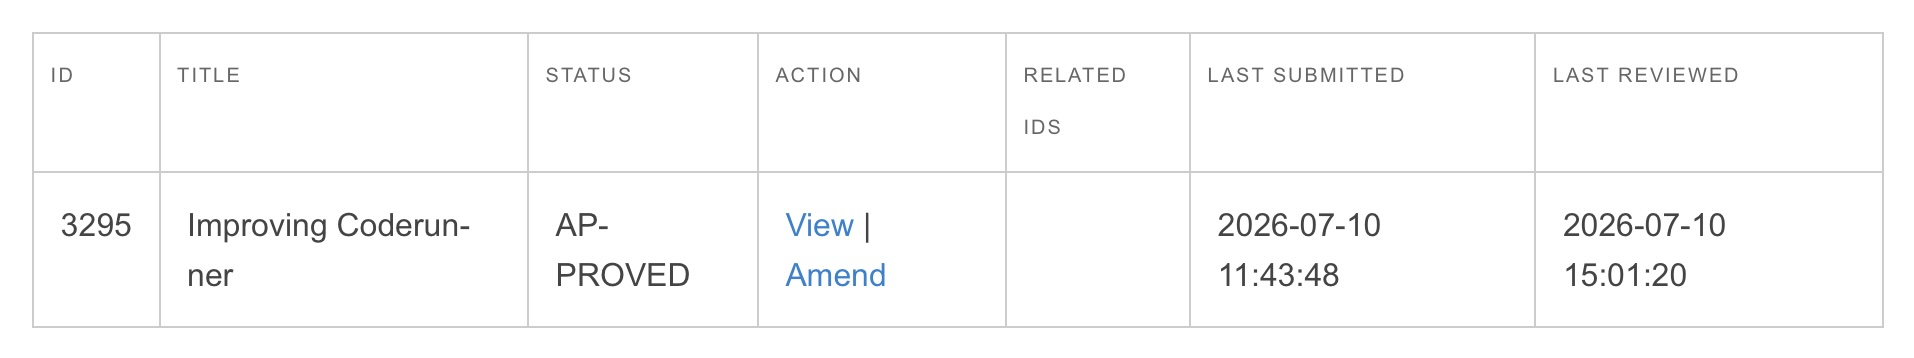
\includegraphics[width=0.7\textwidth]{figs/approval.jpg}
    \caption{Ethical Approval found on the Strathclyde Ethics page}
    \label{fig:ethicsapproval}
\end{figure}

\subsubsection{Participant Information Sheet}
\emph{Github:} \url{https://github.com/michal-skraburski/mono-moodle-docker/blob/main/survey/information/Participant%20Information%20Sheet%20for%20Survey%20of%20Improving%20Coderunner.pdf}


\emph{Microsoft Sharepoint:} \url{https://strath-my.sharepoint.com/:b:/g/personal/michael_skraburski_2022_uni_strath_ac_uk/IQCZ9rzUDisVQ5cogEBKp8NaAZVEz6FbEr3ZcyZ0uesNYtE?e=LWoPEE}
\subsubsection{Consent Form}
\emph{Github:} \url{https://github.com/michal-skraburski/mono-moodle-docker/blob/main/survey/information/consent%20form%20Coderunner.pdf}


\emph{Microsoft Sharepoint:} \url{https://strath-my.sharepoint.com/:b:/g/personal/michael_skraburski_2022_uni_strath_ac_uk/IQBuEWi08Wb9SIbs33qZy9SsASCw3drzVzA__IZTQId0BH0?e=Hem5ae}
 % Add one file per appendix

\end{document}
